\documentclass[12pt]{article}
\usepackage{amsmath}
\usepackage{graphicx} 
\usepackage{geometry}
\usepackage{bm}
\geometry{top=2.0cm,left=2.5cm,bottom=2.0cm,right=2.5cm}
\usepackage{caption}
\usepackage{listings}

\lstset{language=Matlab}
\usepackage[framed,numbered,autolinebreaks,useliterate]{mcode}
\title{\textsf{SABRE: NaI[Tl] scintillators Detector Characterization by Compton Coincidence}}
\author{ Jinnan Zhang\\u6456141@anu.edu.au\and Lindsey Bignell(Superviser)\\lindsey.bignell@anu.edu.au \and Gregory Lane (Supervisor)\\gregory.lane@anu.edu.au\and Andrew Stuchbery (Co-Supervisor)\\andrew.stuchbery@anu.edu.au}
\date{}

\begin{document}
	\maketitle
	\section{Abstract}
	\textbf{The initial purpose of this project is to find the energy capacity of NaI scintillators detector, which will be the mainly used detector in SABRE experiment. In this project, I mainly study the simulated the Compton scattering energy distribution for $^{137}Cs$ source (662kev gamma ray). I was trying to calculate the energy deposited in NaI crystal by comparing the spectrum of  expected Compton scattered Gamma ray and actual scattered gamma ray. Finally, I verified the simulated spectrum of Compton scattering, however, due to the technical difficulties of NaI(Tl) detector, I did not get the capacity information of it.}
	\section{Introduction}
	\subsection{The Background}
	Detecting the dark matter is a both great  and important challenge for  particle- and astro- physics nowadays. The fundamental assumption of Sodium-iodide with Active Background Rejection (SABRE) experiment is that the dark matter is mainly consists of WIMPs (Weakly Interacting Massive Particles). The WIMPs would possibly interact with high purity NaI(Tl) crystals via weak interaction, which leads to a way of detecting dark matter by measuring the nuclear recoil energy following an elastic WIMP scattering off nuclei.
	\subsection{NaI(Tl) Scintillators Detector}
	The NaI(Tl) detector is an essential part of the SABRE. Before the actual experiment, it is necessary to have a clear understanding of NaI(Tl) scintillator. We assume that the Compton scattering of gamma ray with NaI(Tl) as target will help us understanding the property of the detector. The NaI crystal will deposit some energy while interacting with WIMP of dark matter, and this kind of property or capacity	 will be studied in this project.
	\subsection{The Compton Coincidence and HpGe Detector }
	The energy of gamma ray could be  deposited in the sodium iodide crystal, which could be calculated by collect the spectrum of the scattered photons with the help of high purity germanium detector(HpGe). For Compton  scattering, we can calculate  the scattered energy and differential crossing section, combining with the detection efficiency of HpGe detector, we will get an expected gamma ray spectrum. \\
	While experimenting, we only record the signals that appear at both NaI(Tl) detector and HpGe detector at almost the same time($\Delta t << 1\ ms$). This is so called Compton coincidence.
	\subsection{The Basic Geometry Setting of the Detection System}
	The geometry of the detection is pretty straightforward as shown in figure 1:\\
	\begin{figure}[h]
		\centering
		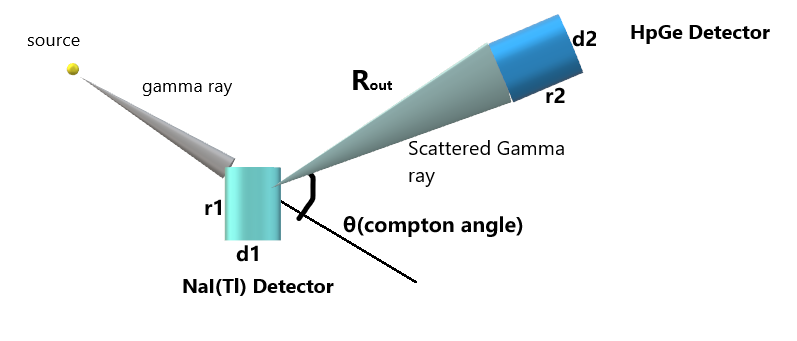
\includegraphics[width=0.7\linewidth]{pic/Basic_Geo_sys}
		\caption{The Basic Experiment Setup for Compton Coincidence}
		\label{fig:basicgeosys}
	\end{figure}\\
	The source here is the radiative source such as $^{137}Cs$ or $^{133}Ba$, which will emit gamma rays.\\	\\
	The $\theta$ here stands for the intersection angle of line defined by source and geometric center of NaI(Tl) detector and line defined by NaI(Tl) center and HpGe detector geometric center.\\
	The parameter r and d are the depth and width of the detectors respectively.
	\section{Python Code Simulation Before Experiment}
	\subsection{Compton Scattering and Differential Crossing Section}
	With basic principle of energy, momenta conservation, the scattered gamma ray energy as function of Compton angle:
	\begin{gather}
		E_{out}=\frac{E_{in}}{1+\frac{E_{in}}{{m_0c^2}}(1-cos\theta)};
	\end{gather} 
	Here $m_0c^2=511keV$ is the mass energy of electron.\\
	The overall experiment will be held in angle range of (0,180) degree, which is plotted as :
	\begin{figure}[h]
		\centering
		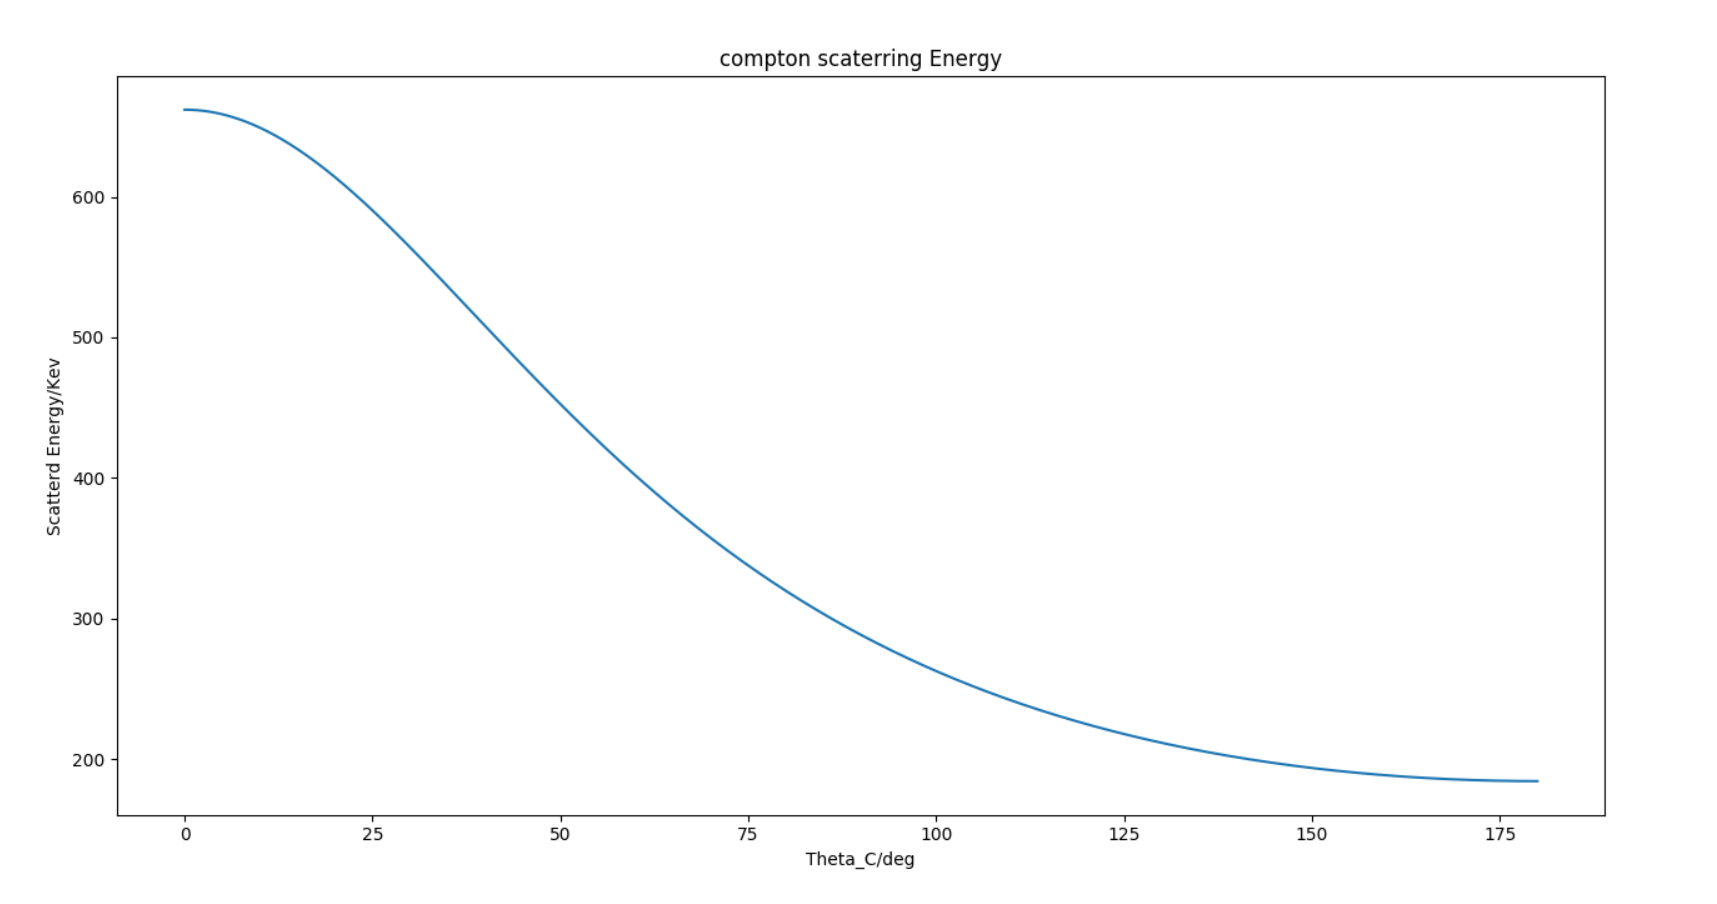
\includegraphics[width=0.7\linewidth]{pic/Scattered_E_simulation}
		\caption{The Compton Scattered Energy-Scattering angle}
		\label{fig:scatteredesimulation}
	\end{figure}\\
	Notice that the scattered energy as function of $\theta_C$ is monotonic decreasing, which could help us better perform the overall simulation about energy distribution.\\
	
	And the probability of scattered to a particular angle $\theta$ by Klein-Nishina formula:
	\begin{gather}
		\frac{d\sigma_{c,e}}{d\Omega}=r_0^2(\frac{1}{1+\alpha(1-cos\theta)})^2(\frac{1+cos^2\theta}{2})(1+\frac{\alpha^2(1-cos\theta)^2}{(1+cos^2\theta)[1+\alpha(1-cos\theta)]});\\
	\alpha=\frac{h\nu}{m_0c^2};
	\end{gather}
	Here,$\ r_0=\frac{e^2}{4\pi \epsilon_0m_0c^2}=2.818\times 10^{-15}\ m.$  is the classical electron radius. \\
	While simulating, I normalized the differential crossing section to scattering relative probability from raw differential crossing section data being divided by the greatest crossing section. This process will not give a sum-1 distribution but a relative probability of occurrence donate as $P_{diff\_Cross}$:
	\begin{figure}[h]
		\centering
		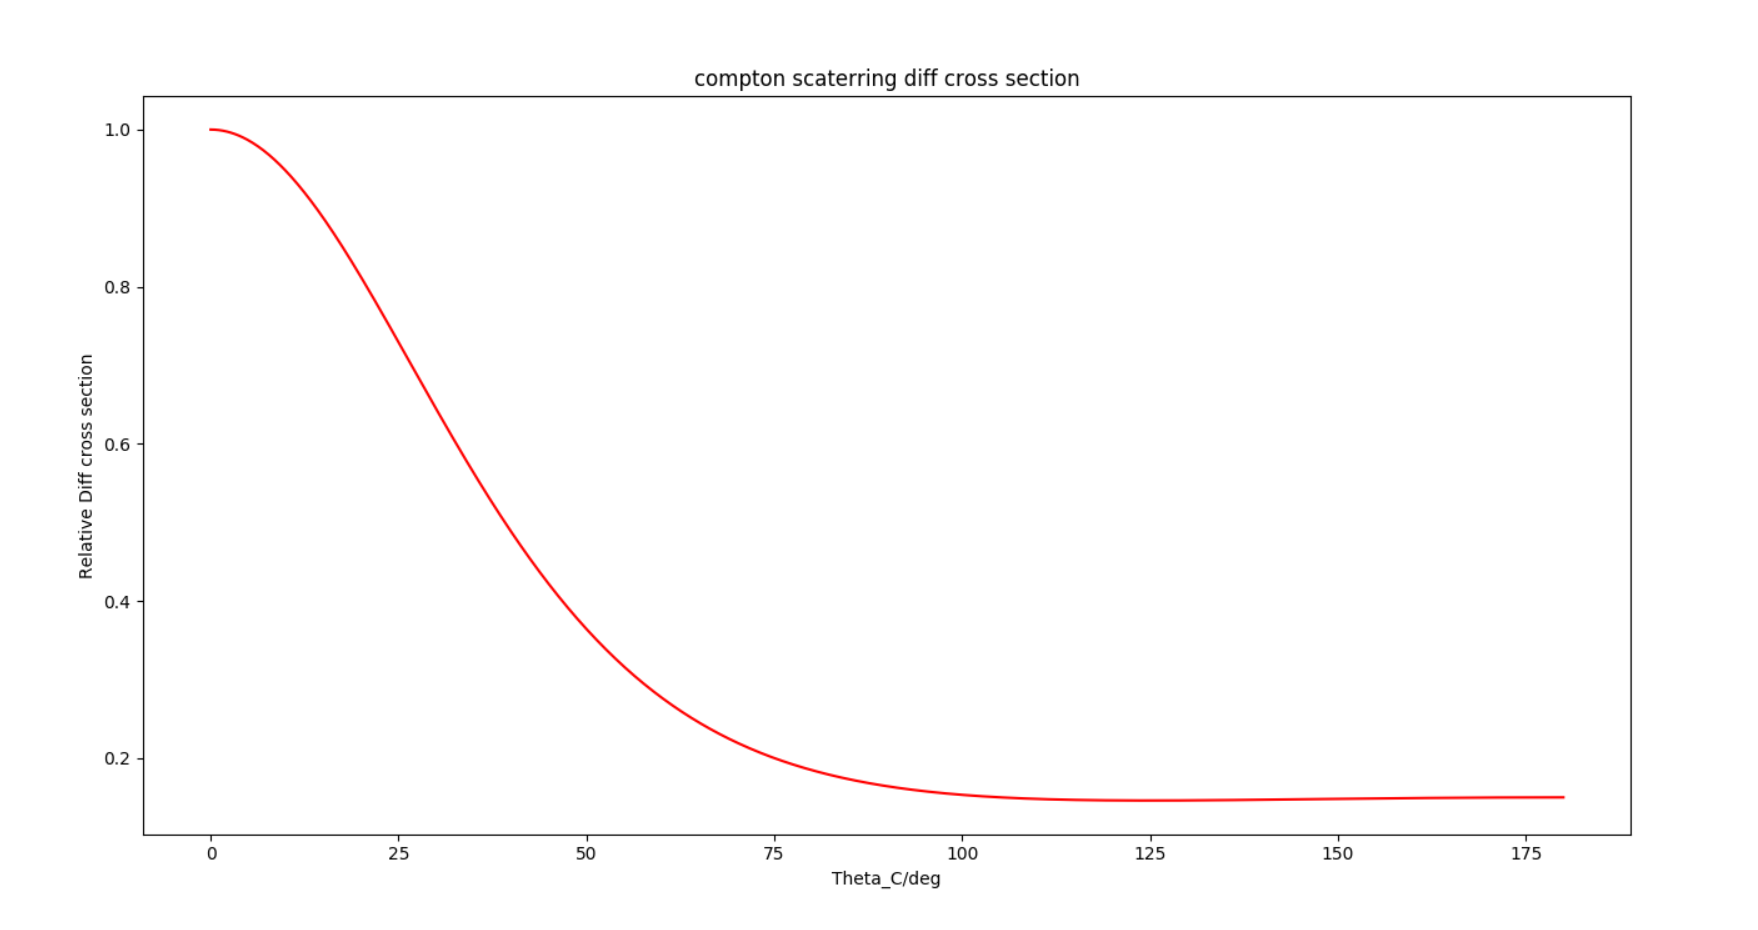
\includegraphics[width=0.7\linewidth]{pic/Scattered_diffCS__simulation}
		\caption{The Relative Probability Distribution of Scattered Angle}
		\label{fig:scattereddiffcssimulation}
	\end{figure}
	
	
	\subsection{HpGe Detector Detection Efficiency}
	The HpGe detector we are using to collect the scattered spectrum is based on the light will interact with the Ge crystal.  The interaction probability will result in the detection efficiency, which could be evaluated by :\\
	The light intensity with the initial value $I_0$ and I is the light intensity after going through the metrical with depth t as:
	\begin{gather}
	I=I_0e^{-\mu t}
	\end{gather}
	Here $\mu$ is the coefficient, and is the function of the light energy.\\
	Thus, the interacting probability P is :
	\begin{gather}
	P_{int}=\frac{I_0-I}{I_0}=1-exp(-\mu t)
	\end{gather}
	Since $\mu$ is function of light energy, light energy is scattering angle; and t is function of $\theta_C$.
	\begin{gather}
		P_{int}=1-exp(-\mu(E) t(\theta_C);\\
		\to P_{int}=P_{int}(\theta_C).
	\end{gather} 
	The coefficient could be  found on web site of NIST:\\$https://physics.nist.gov/cgi-bin/Xcom/xcom2 $\\
	There is only some  discrete values of absorption coefficient. Since I want to get the whole interaction wave form of a range of energy, fitting the data to expansion function by Origin:
	\begin{gather}
		\mu=exp(a+bE_\gamma+cE_\gamma^2);\\
		a=5.28707\pm 0.08149;\\
		b=-0.05223\pm 0.00158;\\
		c=3.7691\times 10^{-5}\pm 4.28757\times 10^{-6}.
	\end{gather}
	The processing of data fitting is shown as following:
	\begin{figure}[h]
		\centering
		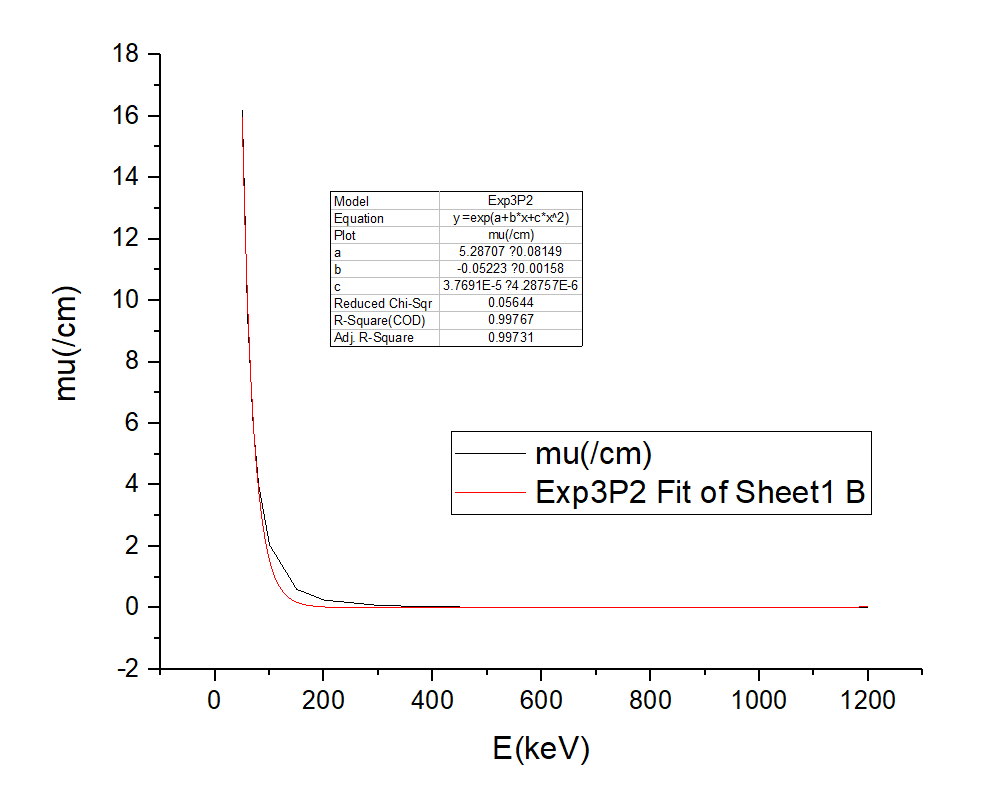
\includegraphics[width=0.7\linewidth,height=0.2\textheight]{pic/fit_mu}
		\caption{Origin data fit of $\mu$ }
		\label{fig:fitmu}
	\end{figure}\\
	The data is not perfectly fitted, but it is sufficiently for us since the energy range of the detection is almost (200,600).
	
	\subsection{The Overall Distribution}
	The expected distribution $P_{expect}$ should be the combination of scattering and absorption as:
	\begin{gather}
		P_{expect}=P_{diff\_Cross}\cdot P_{int};
	\end{gather}
	is function of geometry of the system.\\
	The simulation python 3 code is in the appendix.\textbf{ For simplicity, the NaI(Tl) detector is regarded as a point target, and only the single scattering is considered.}\\
	 With parameters as :
	\begin{gather}
		R_{out}=10.000cm;\\
		d_2=r_2=5.000cm;\\
		E_{in}=662kev;\\
		\theta_{main}=80deg;
	\end{gather}
	The simulation will gives the overall relative probability distribution waveform of scattered energy in figure 5:
	\begin{figure}[h]
		\centering
		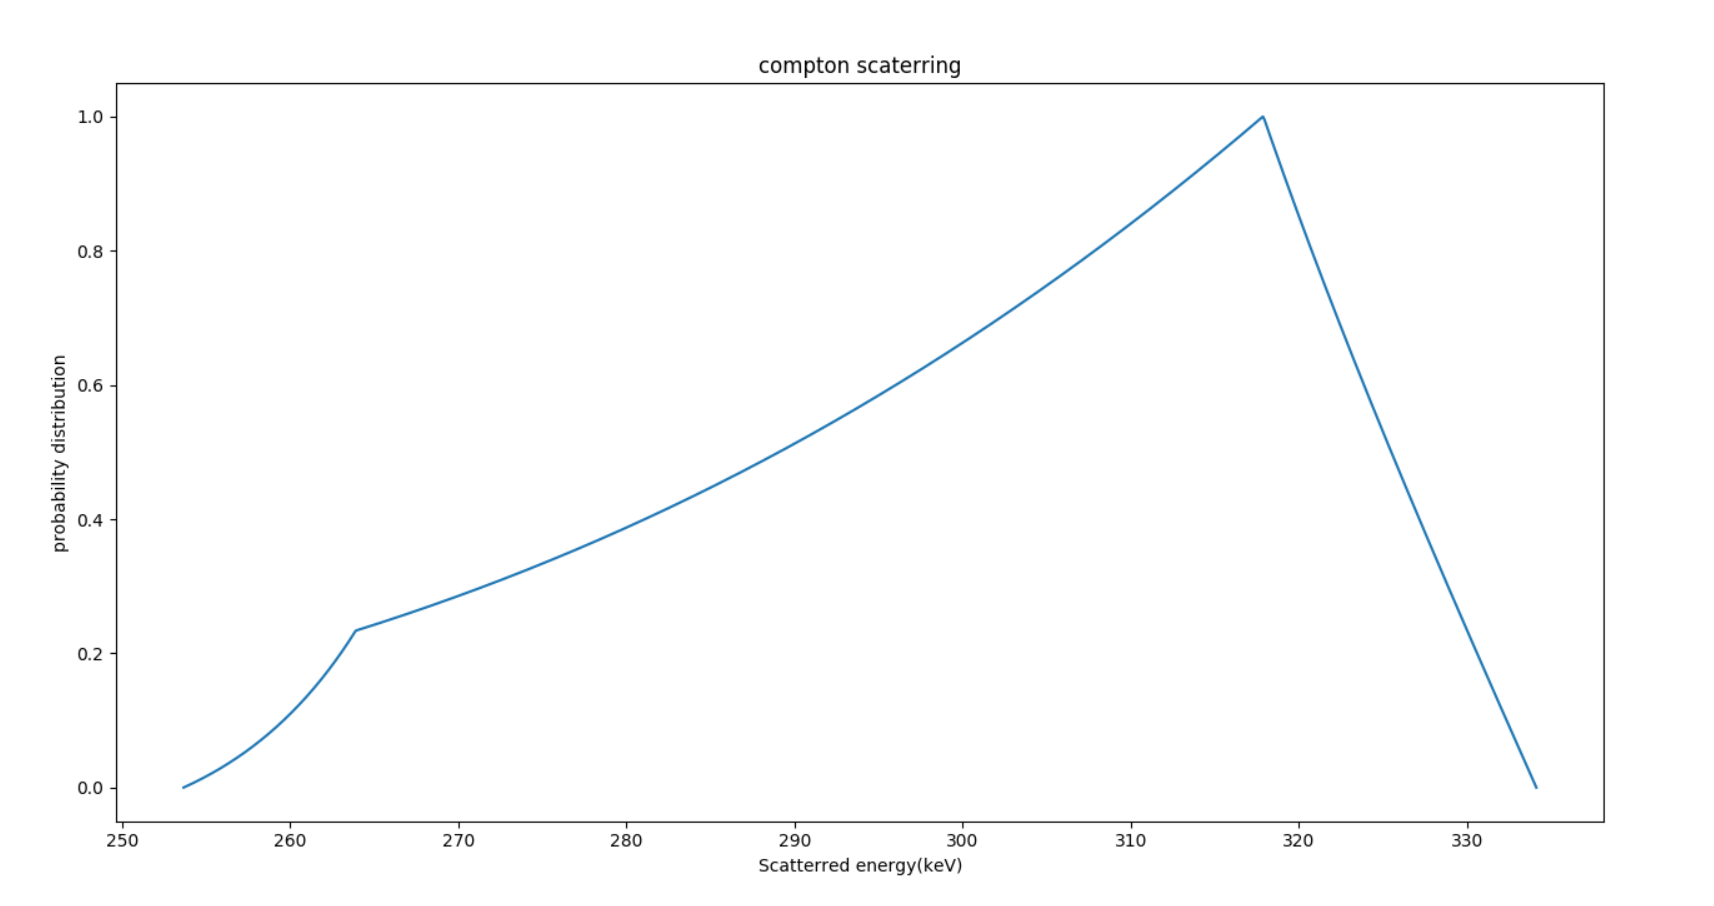
\includegraphics[width=0.7\linewidth]{pic/com_scat_R10_5x5_662kev_80deg}
		\caption{Scattered Energy Relative Distribution}
		\label{fig:comscatr105x5662kev80deg}
	\end{figure}\\
	Notice that the detection efficiency of HpGe detector adds some shape factor into the distribution waveform.
	\section{Experiment Setup}
	\subsection{Experiment Setup and Data Collection}
	The photoelectric pulse from the NaI(Tl) detector and HpGe detector will be recorded by CAEN DT5720D digitizer with binary files. \\
	The signal from NaI(Tl) detector will be directly recorded by the digitizer. For HpGe detector, however, the signal from the detector will be amplified by the amplifier first and then integrated by the  integrator. Thus, the data we get from the digitizer of NaI(Tl) detector will be the photoelectric pulse waveform and we need to do further integration to get the charge and energy. As for the data from the HpGe detector, the uncalibrated energy could be extracted from the data file by find the maximum of the waveform.\\
	The basic experiment setup is shown in figure6:
	\begin{figure}[h]
		\centering
		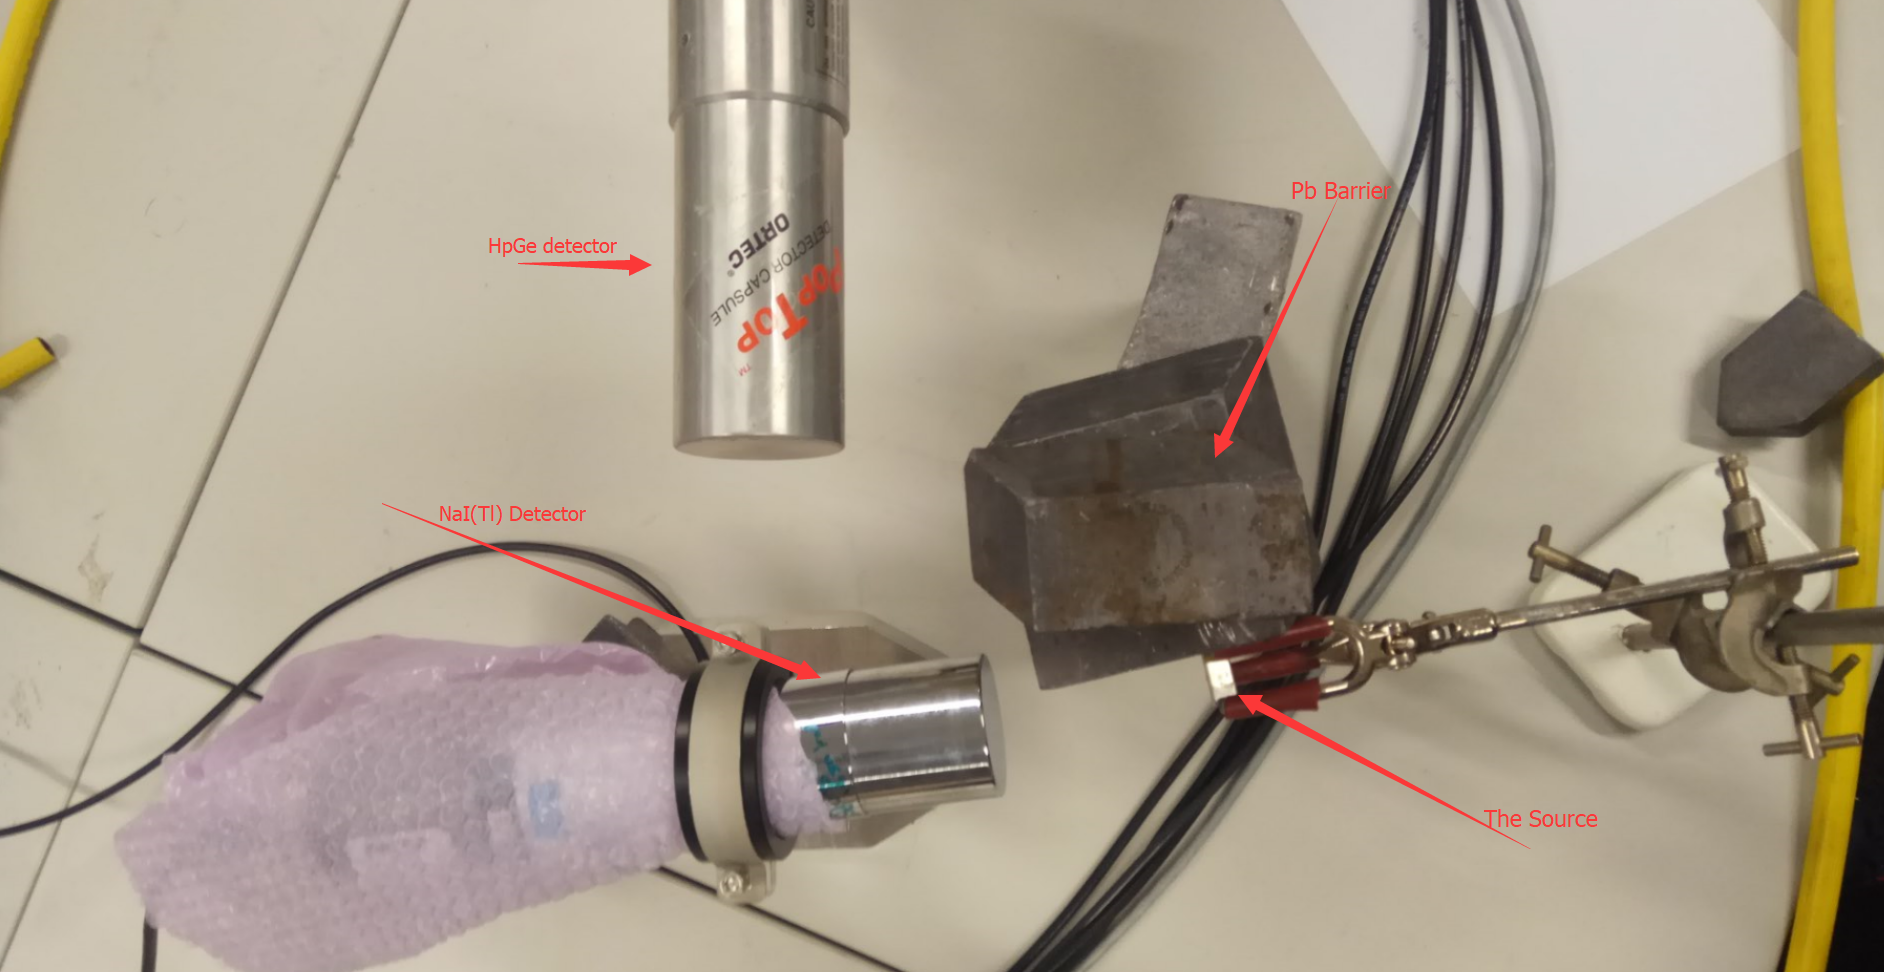
\includegraphics[width=0.7\linewidth, height=0.2\textheight]{pic/experiment_lab_set}
		\caption{The Actual Setup of the Lab at Beginning}
		\label{fig:experimentlabset}
	\end{figure}\\
	Here the high voltage is negative 1500V for NaI(Tl), negative 3600V for HpGe. 
	\subsection{The Data Analysis Method}
	The example wave form I got from the NaI(Tl) detector of the coincidence experiment is shown in figure 7:
	\begin{figure}[h]
		\centering
		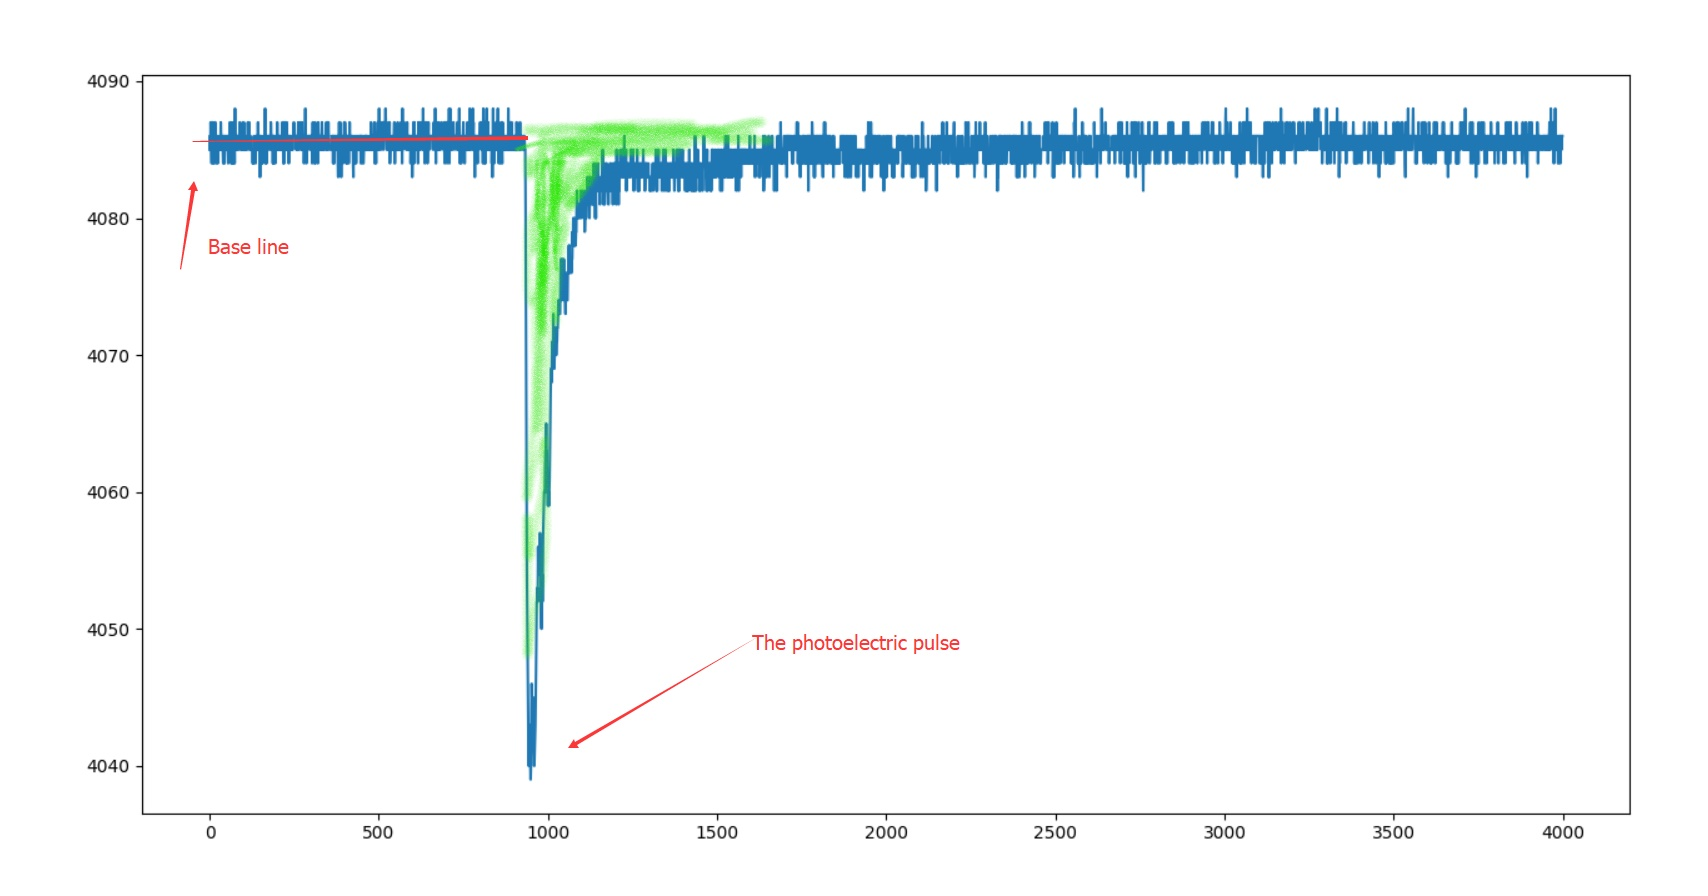
\includegraphics[width=0.7\linewidth,height=0.2\textheight]{pic/Inkedwaveform_NaI_LI}
		\caption{The photoelectric pulse waveform of NaI(Tl) detector}
		\label{fig:waveformnai}
	\end{figure}\\
	As the gamma ray incoming  into the NaI(Tl) Scintillators detector, the detector will generate electrons with energy proportional to the gamma ray energy. The electrons be amplified to become a negative pulse signal, which is we got in Figure 7. The area below the average  baseline (The red line in Figure 7) and enclosed by the pulse waveform gives the uncalibrated energy(i.e. The green are in Figure7), which has a linear relationship with the actual energy of the gamma ray.\\
	The hardware integrated waveform of HpGe detector is shown in figure 8:
	\begin{figure}[h]
		\centering
		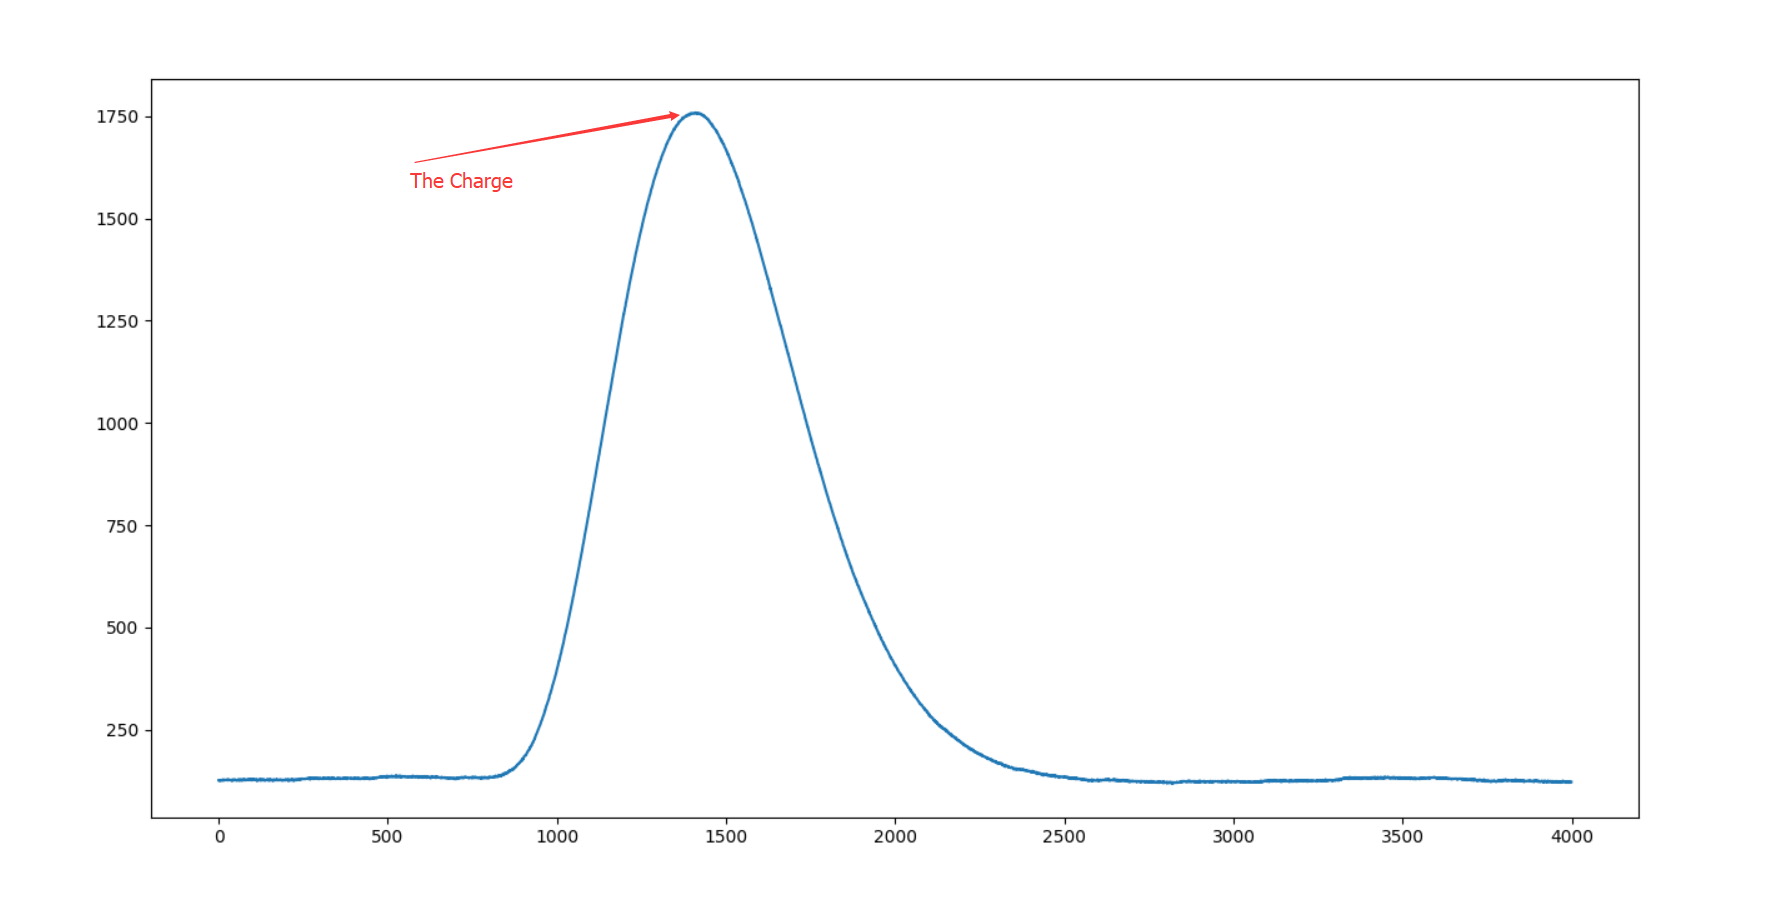
\includegraphics[width=0.7\linewidth,height=0.15\textheight]{pic/waveform_HpGe}
		\caption{The Integrated Waveform of HpGe Detector}
		\label{fig:waveformhpge}
	\end{figure}\\
	The peak value of the waveform is just the uncalibrated energy value.\\
	The python 3 code to extract the data is also in the appendix.
	\subsection{Energy Calibration}
	The detectors will give us the charge of the photoelectrons, however, we need to do further energy calibration to specify the energy of the gamma ray photons received in the coincidence experiment.\\
	The method of calibration is: set the same lab condition as coincidence except the geometry of the detectors and source, find out the relation of the uncalibrated energy calculated from the detector data  and the actual energy of the gamma ray. Once the relation is clear, apply it to the coincidence experiment to get the actual energy plot.\\
	Consider the result  we got in the simulation, the energy range of coincidence experiment will be at about (200,400)keV, and we are not sure of that the zero of the uncalibrated energy will be the zero energy point of the gamma ray. Select the multiple peak radioactive source $^{133}Ba$. The gamma rays intensity distribution of $^{133}Ba$ from \\\textbf{http://www.spectrumtechniques.com/products/sources/ba-133} is shown in\\Table 1:
	\begin{table}[ht]
		\centering
		\begin{tabular}{|c|c|}\hline
			Energy(kev)& Intensity(\%)\\\hline
			53.161&	2.199\\
			79.621&	2.62\\
			80.997&	34.06\\
			160.613&	0.645\\
			223.398	&0.45\\
			276.398	&7.164\\
			302.853&	18.33\\
			356.017	&62.05\\
			383.851	&8.94\\\hline
		\end{tabular}
		\caption{The Gamma ray Intensity distribution}
	\end{table}\\
	Notice that the 356kev gamma ray dominates the gamma ray spectrum of $^{133}Ba$. \\
	I did the energy calibration measurement with the geometry shown in Figure 9:
	\begin{figure}[h]
		\centering
		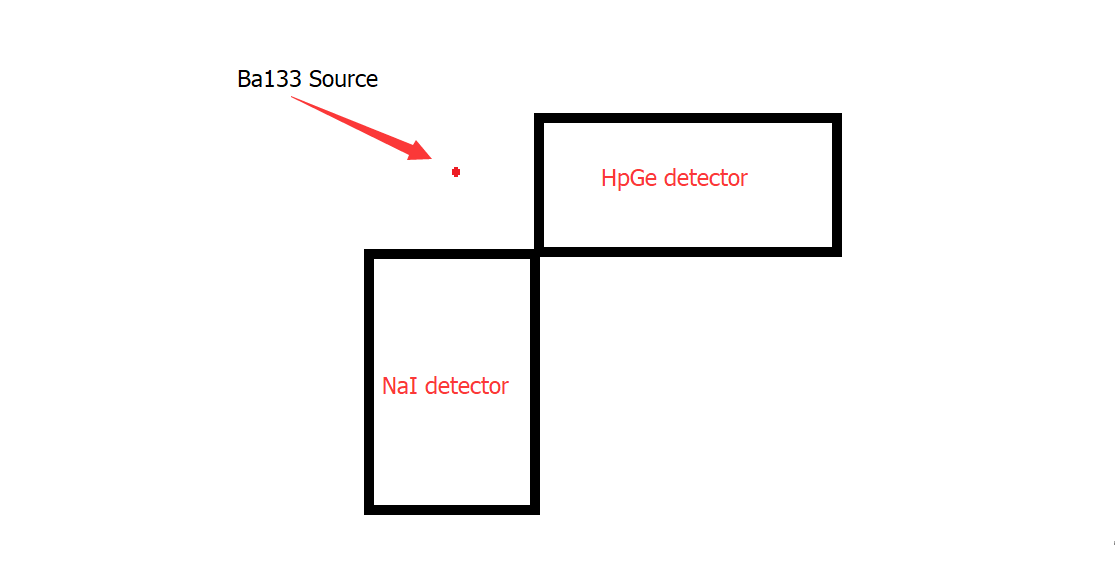
\includegraphics[width=0.7\linewidth, height=0.15\textheight]{pic/calibration_geo}
		\caption{The Energy Calibration Experiment Geometry Setup}
		\label{fig:calibrationgeo}
	\end{figure}\\
	The center of NaI(Tl) detector and HpGe are on the same plane.
	\subsubsection{HpGe Detector}
	According to the actual  uncalibrated energy of $^{133}Ba$ gamma ray  and the plot peak in figure 10:
	\begin{figure}[h]
		\centering
		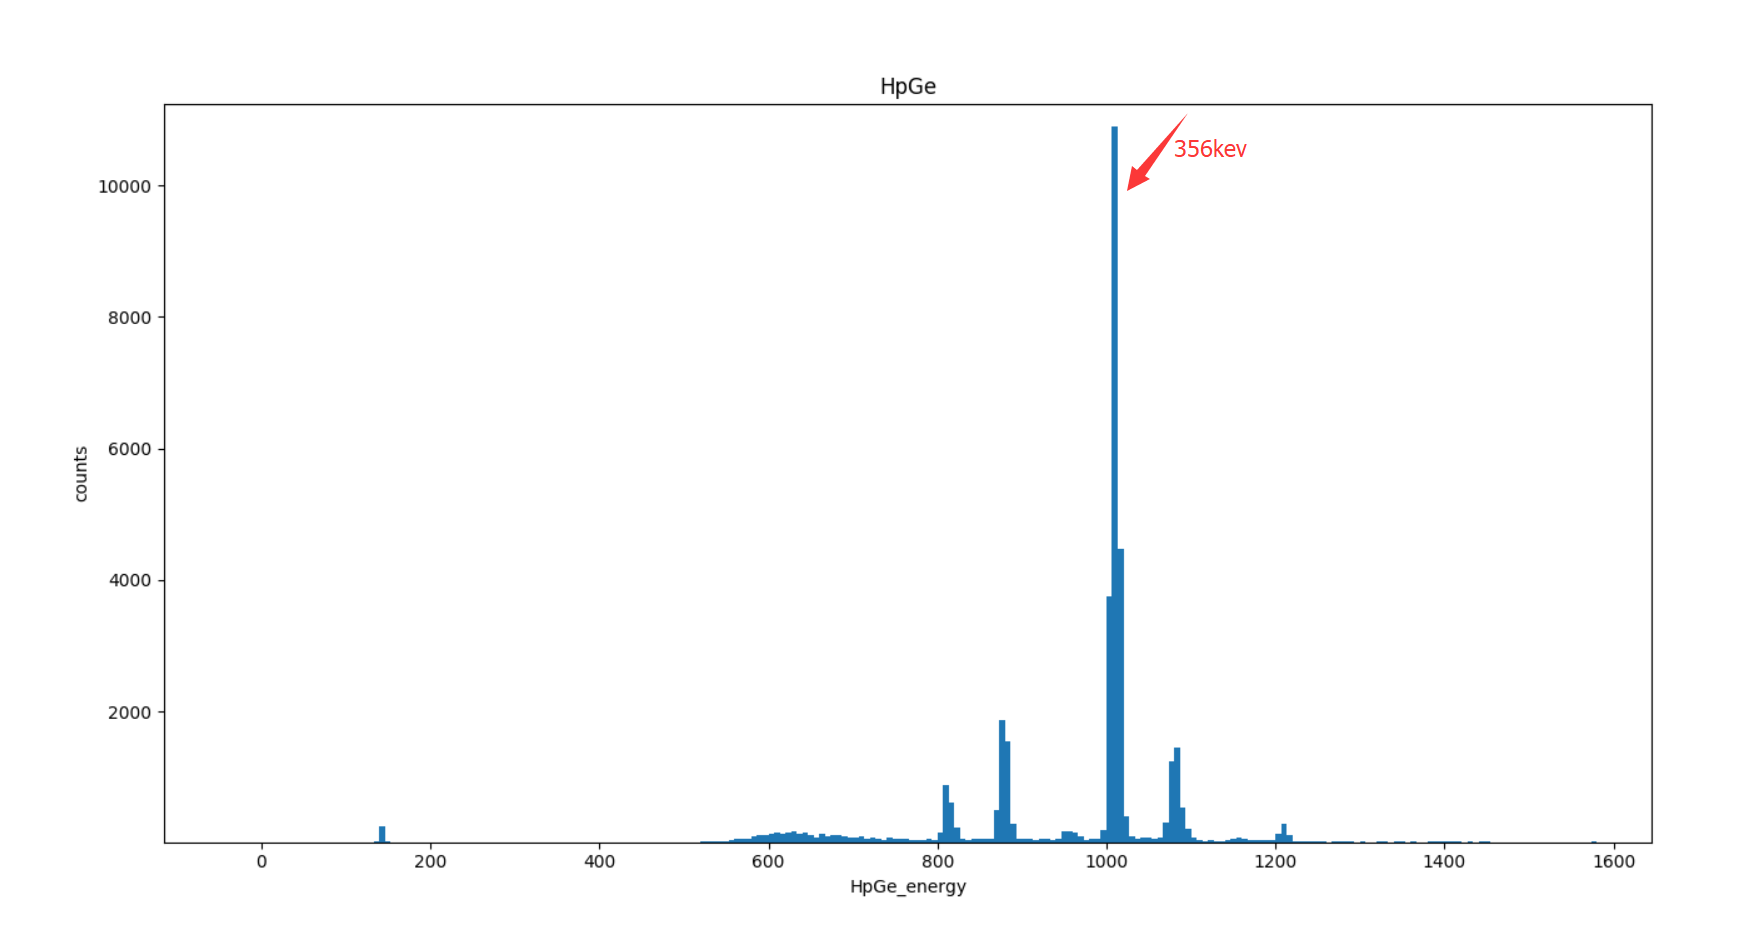
\includegraphics[width=0.7\linewidth, height=0.2\textheight]{pic/uncalibrated_Ba133_HpGe}
		\caption{Uncalibrated Gamma Spectrum of $^{133}Ba$.}
		\label{fig:uncalibratedba133hpge}
	\end{figure}\\
	The approximately  calibration function of HpGe detector:
	\begin{gather}
		E_{HpGe}=\frac{x\cdot 356}{947};
	\end{gather}
	In (17), x is the value of uncalibrated energy calculated from the hardware integration data. 
	\subsubsection{NaI Detector}
	On energy calibrating of the NaI(Tl) detector, we met lots of problem:\\
	1.There is not multiple peak on the uncalibrated spectrum of $^{133}Ba$;\\
	2.There are still plenty of charge counts around 0 for even no source experiment;\\	
	The spectrum for no source NaI(Tl) detector:
	\begin{figure}[h]
		\centering
		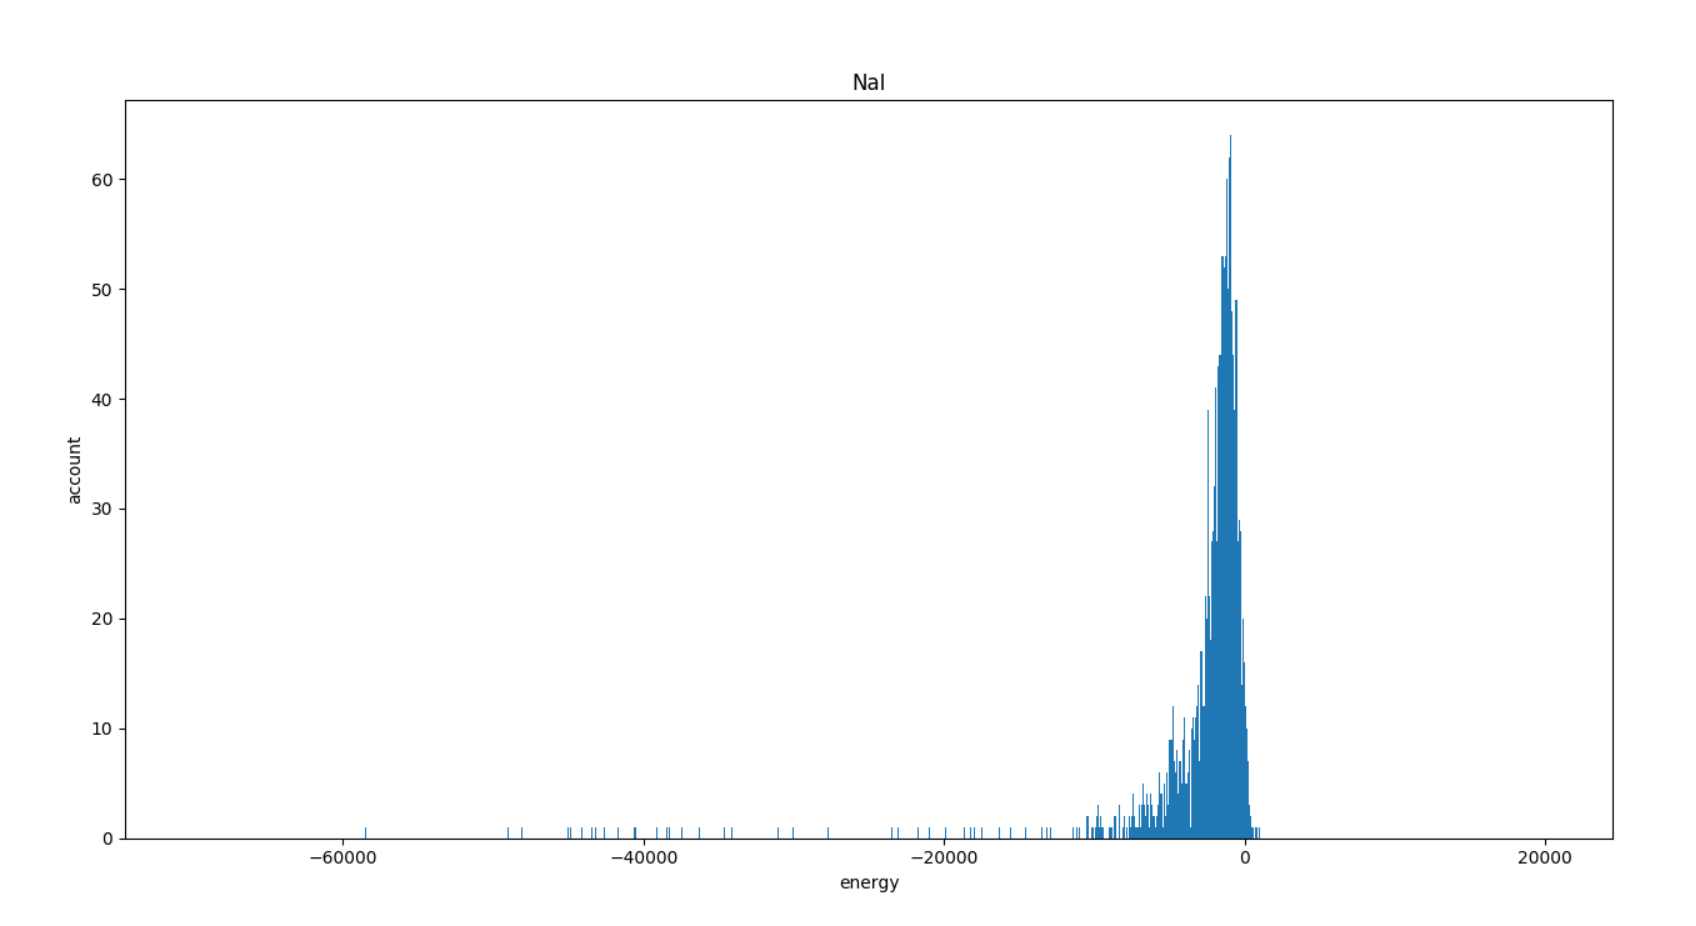
\includegraphics[width=0.7\linewidth, height=0.2\textheight]{pic/NO_source_NaI}
		\caption{No Source NaI(Tl) With Threshold 4025}
		\label{fig:nosourcenai}
	\end{figure}\\
	Notice that there are not much cunt for such circumstance, which would not influence the coincidence result and mostly are noise.\\ 
	The reason for not multiple peak is the threshold is not proper for the experiment.\\
	After further adjustment to the trigger threshold of DT, the calibration data in figure12:
	\begin{figure}[h]
		\centering
		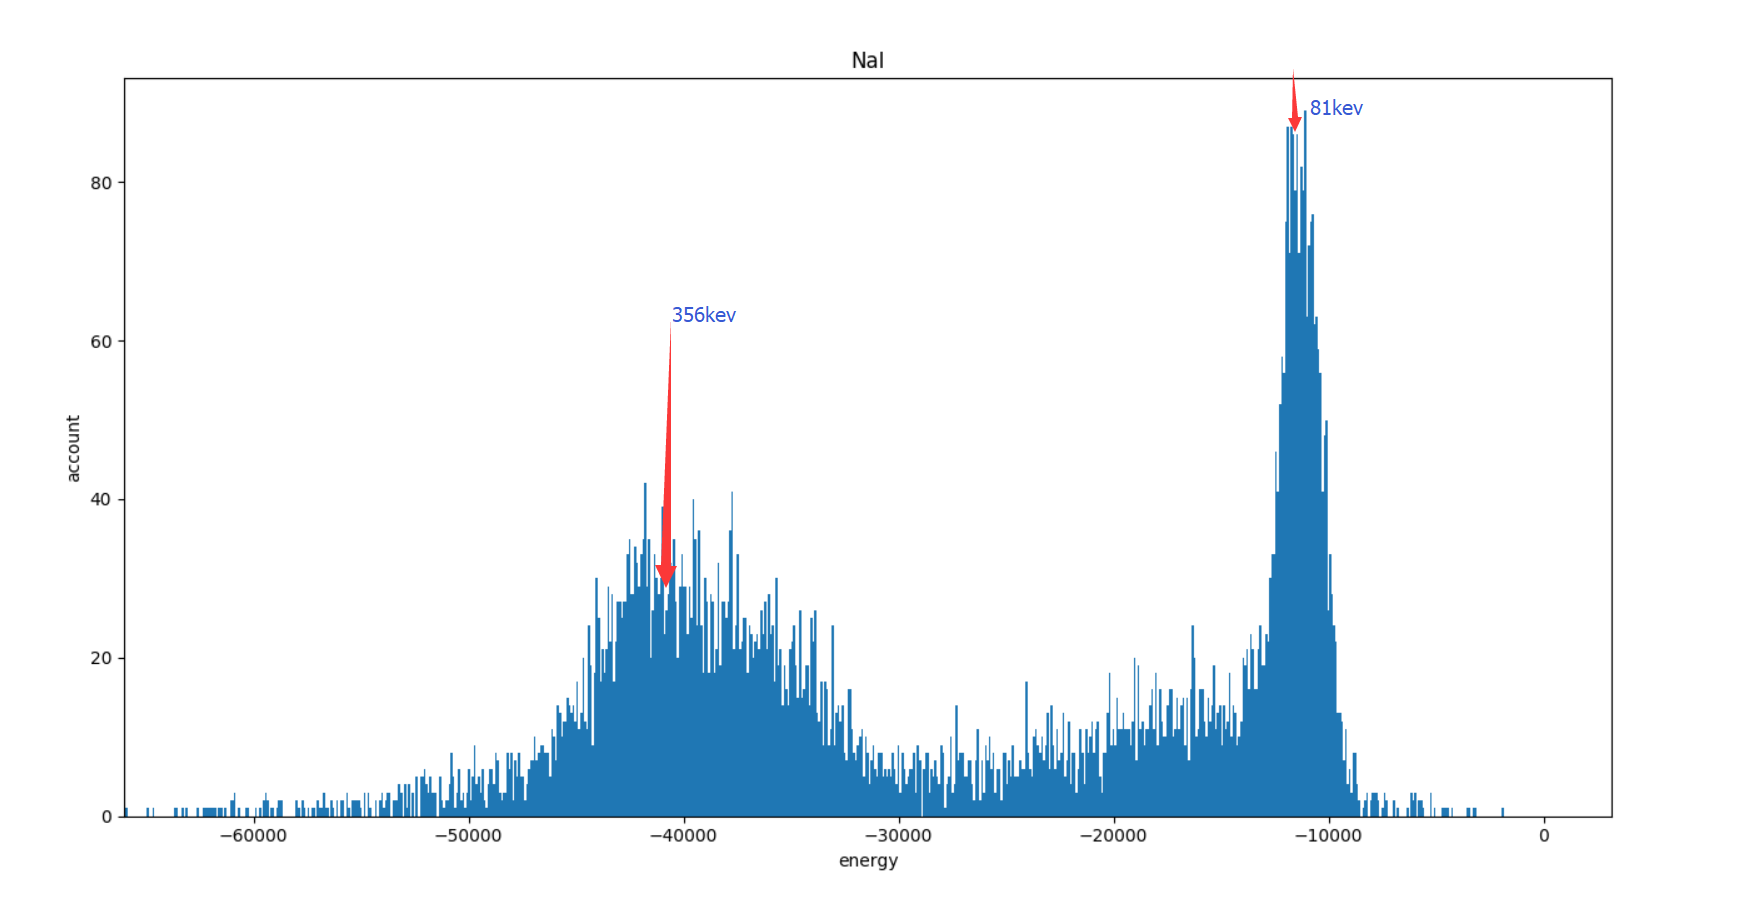
\includegraphics[width=0.7\linewidth, height=0.2\textheight]{pic/NaI_calibration}
		\caption{The Calibration Data for NaI Detector}
		\label{fig:naicalibration}
	\end{figure}
	The calibration function for NaI(Tl) detector:
	\begin{gather}
		E=-6.7+0.0785\cdot x;
	\end{gather}
	Which infers that the zero of uncalibrated spectrum is not actual zero energy.
	
	\subsection{Coincidence Experiment}
	The coincidence experiment will use the radioactive source $^{137}Cs$ to emit the gamma ray.\\
	At the beginning, the experiment geometry was setup as the parameters of following in figure 13 :
	\begin{figure}[h]
		\centering
		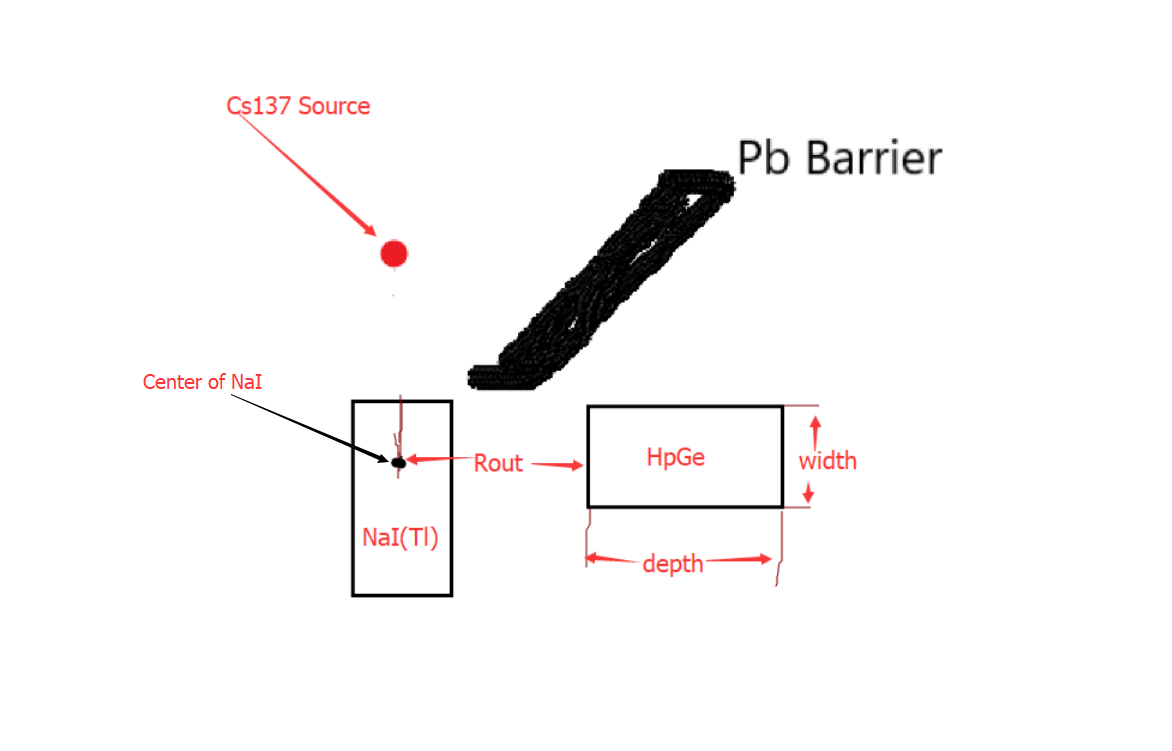
\includegraphics[width=0.7\linewidth, height=0.25\textheight]{pic/Cs_137_far_geo1}
		\caption{The Geometry of 1st Coincidence Experiment}
		\label{fig:cs137fargeo1}
	\end{figure}
	\begin{gather}
		R_{out}=4.532cm;\\
		depth2=7.290cm
		r_2=7.000cm;\\
		E_{in}=662kev;\\
		\theta_{main}=90deg;
	\end{gather}
	But the coincidence events are too rare as shown in figure 14:\\\\
	\begin{figure}[h]
		\centering
		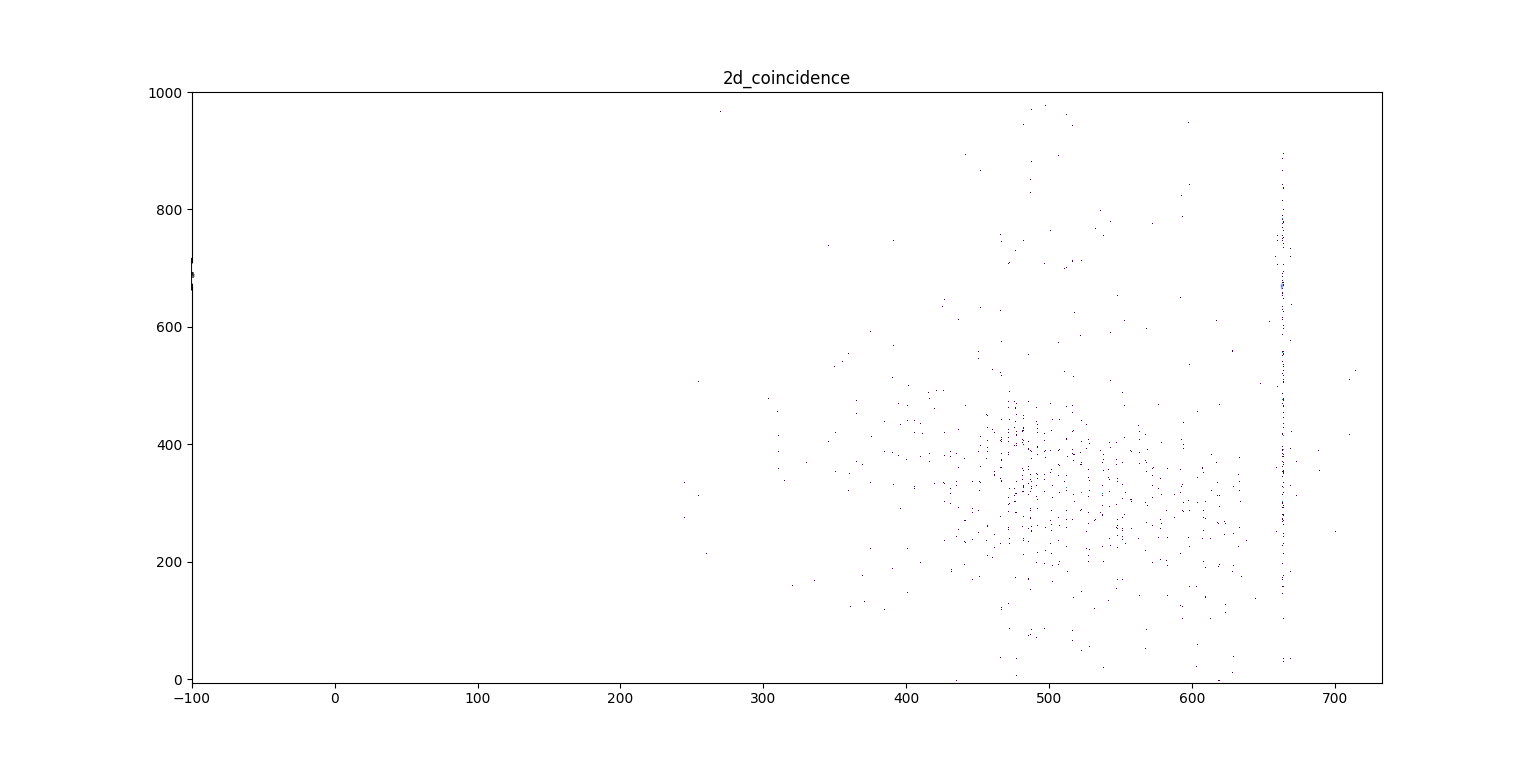
\includegraphics[width=0.7\linewidth, height=0.2\textheight]{pic/Figure_3_coin}
		\caption{The 1st Geometry Coincidence Data}
		\label{fig:figure3coin}
	\end{figure}\\
	 In the plot, the scattering event points are too sparse to recognize the coincidence events.\\
	 Good news here is that the scattered energy of the gamma ray, which was collect by HpGe detector, met the expectation well in Figure 15:\\
	\begin{figure}[h]
		\centering
		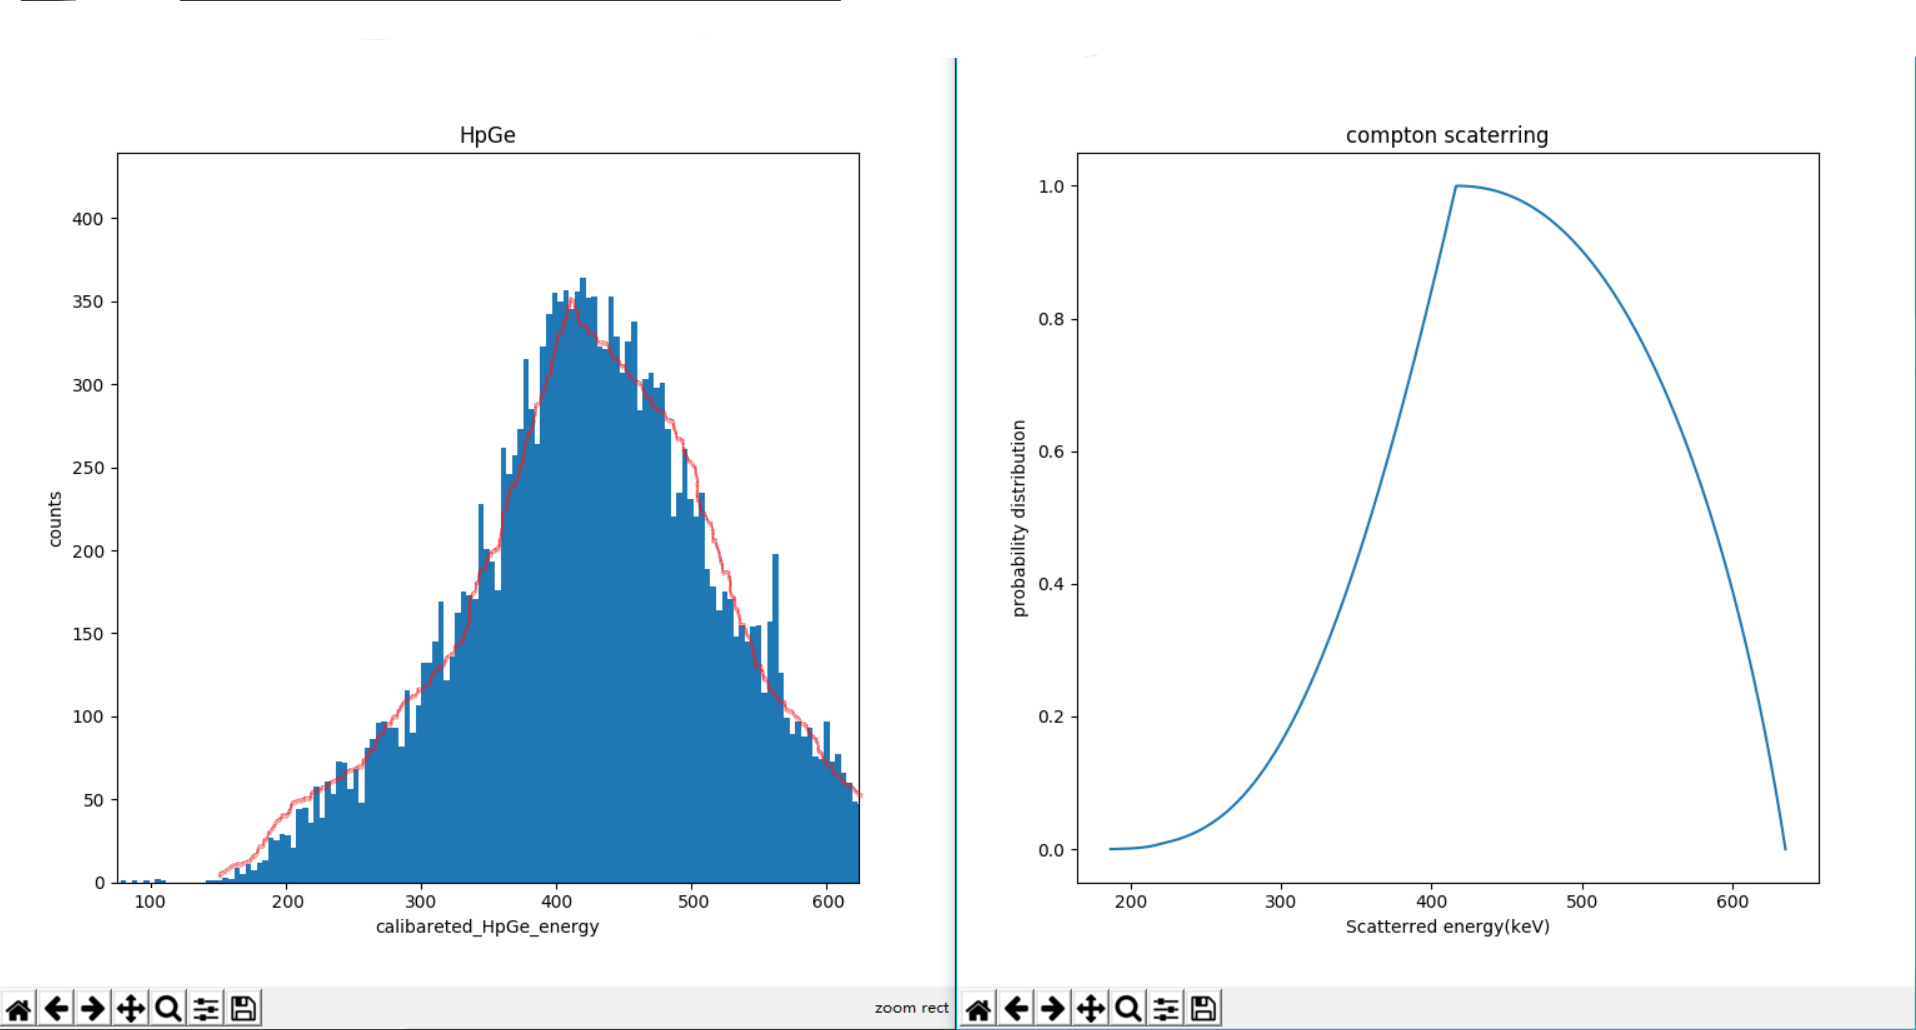
\includegraphics[width=0.7\linewidth, height=0.15\textheight]{pic/HpGe_energy_waveform_calib}
		\caption{The Scattered Energy Spectrum As Expected}
		\label{fig:hpgeenergywaveformcalib}
	\end{figure}\\
	 The trend line of the experiment spectrum(red line on the left) suits the simulation result well, which credit the previous simulation work.\\
	 For more coincidence events, the geometry was adjust to the setup in Figure 16:
	 \begin{figure}[h]
	 	\centering
	 	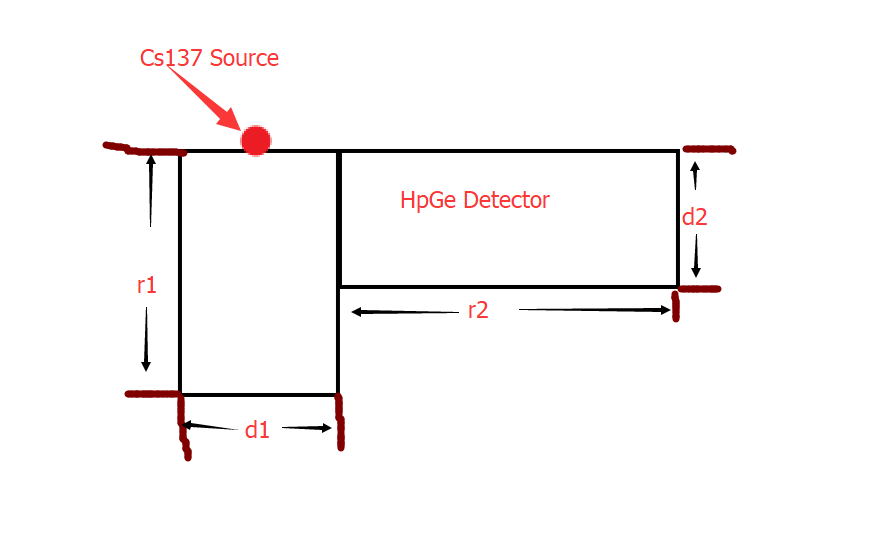
\includegraphics[width=0.7\linewidth, height=0.25\textheight]{pic/Cs_137_close_geo}
	 	\caption{Closer Geometry of Coincidence Experiment}
	 	\label{fig:cs137closegeo}
	 \end{figure}\\
	 Under this geometry, the parameters are:
	 \begin{gather}
	 	R_{out}=\frac{1}{2}d_1=28.24mm=2.824cm;\\
	 	\theta_{main}=90deg=\pi /2;
	 \end{gather}
	The simulation result and HpGe detector spectrum cooperation in Figure 17:
	\begin{figure}[h]
		\centering
		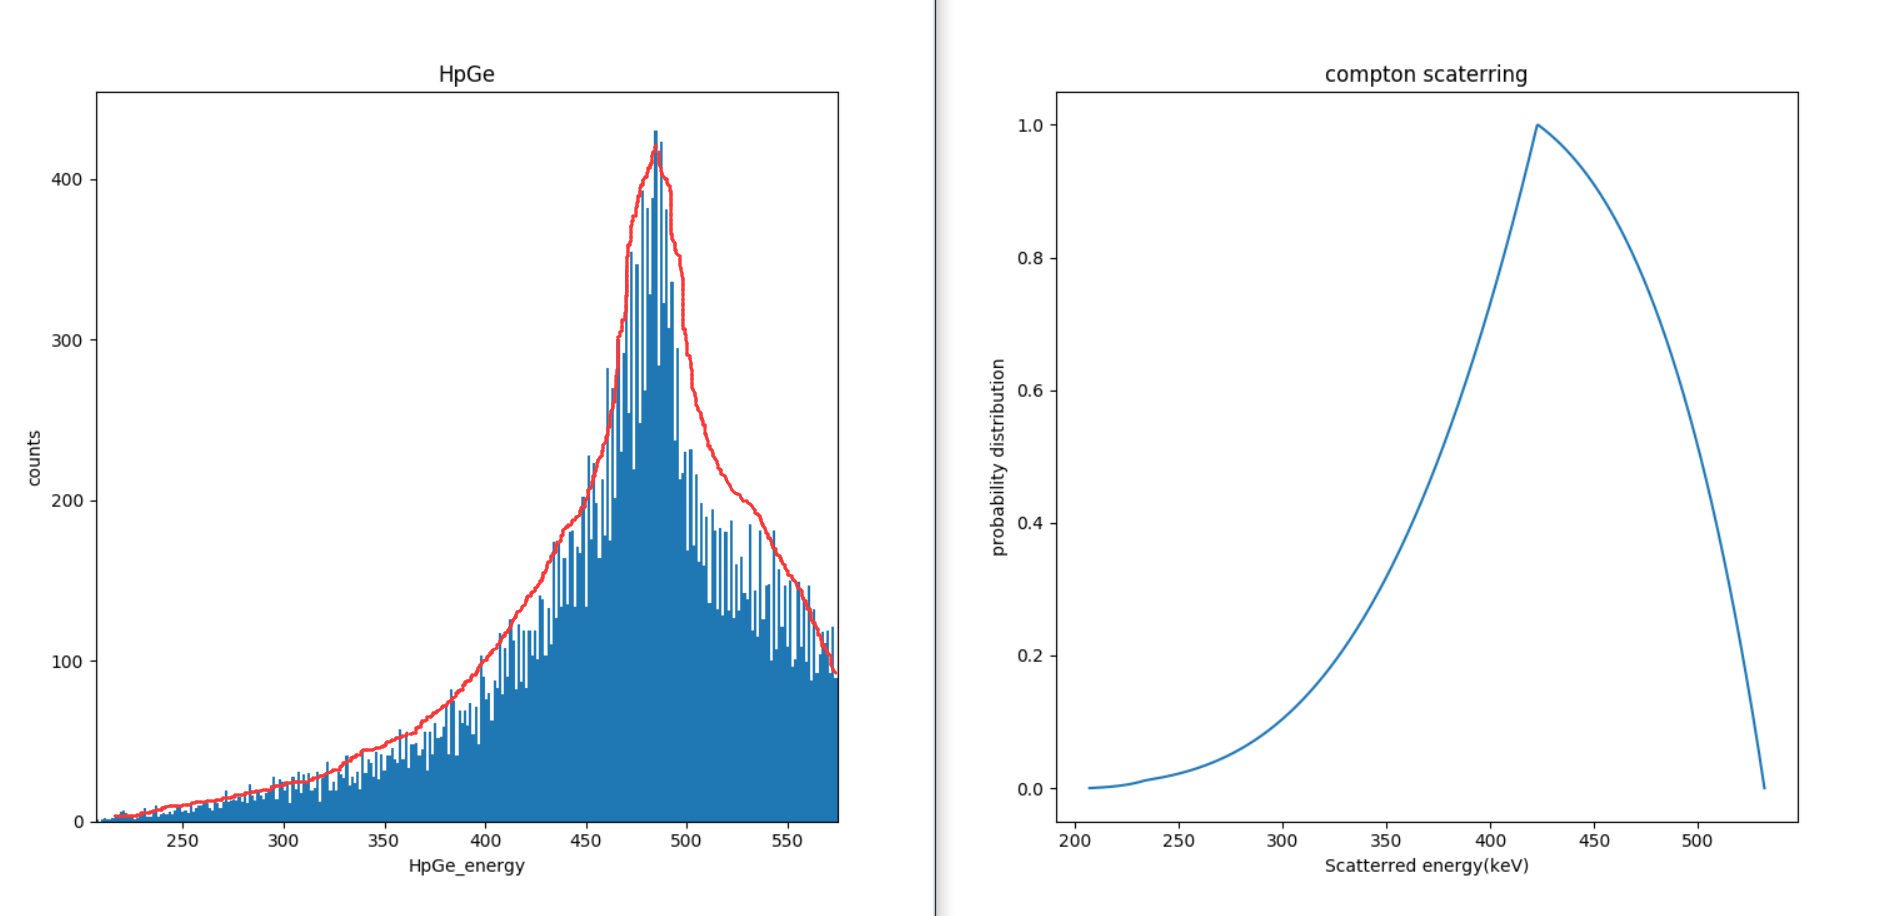
\includegraphics[width=0.7\linewidth, height=0.2\textheight]{pic/compration_HPGe_simulation}
		\caption{The HpGe Spectrum for 2nd Geometry Coincidence Experiment}
		\label{fig:comprationhpgesimulation}
	\end{figure}\\
	The experiment waveform around the peak is a little different from the simulation result, but mostly the same. The waveform  difference is out of the energy deposited in the NaI detector. And there is a peak at 662kev for the directly incidence gamma ray.\\
	The combination events histogram for two detectors in Figure 18:\\
	\begin{figure}[h]
		\centering
		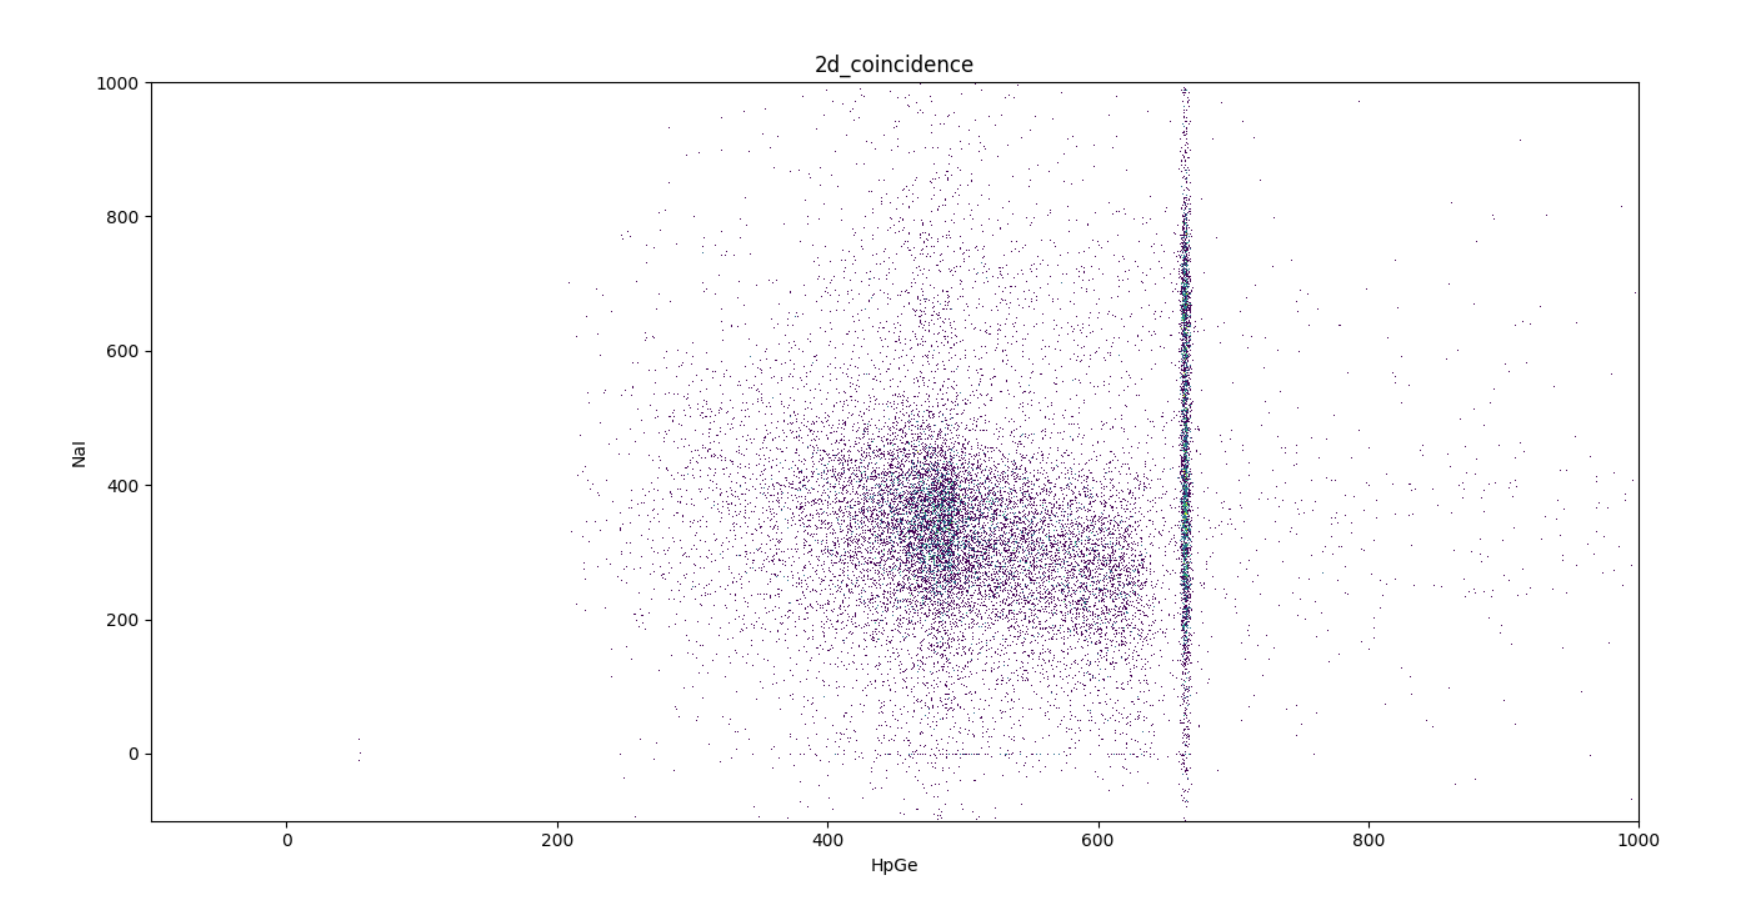
\includegraphics[width=0.7\linewidth, height=0.4\textheight]{pic/Coin_hist_2nd_Geo}
		\caption{Coincidence Experiment: Combination Histogram for Two Detectors}
		\label{fig:coinhist2ndgeo}
	\end{figure}\\
	The vertical line in Figure17 is the 662 kev gamma ray. \\ 
	In the plot, there are more coincidence events, however, we can't see the curve we expected. Our expectations are:\\
	\romannumeral1.) If there is no energy deposited in NaI crystal, there will be a straight line from (0,662) to (662,0) (blue line in Figure 18);\\
	\romannumeral2.) If there is some energy deposited in NaI crystal, according to the conservation of energy, there will be a curve (Green curve) as shown in Figure 19:
	\begin{figure}[h]
		\centering
		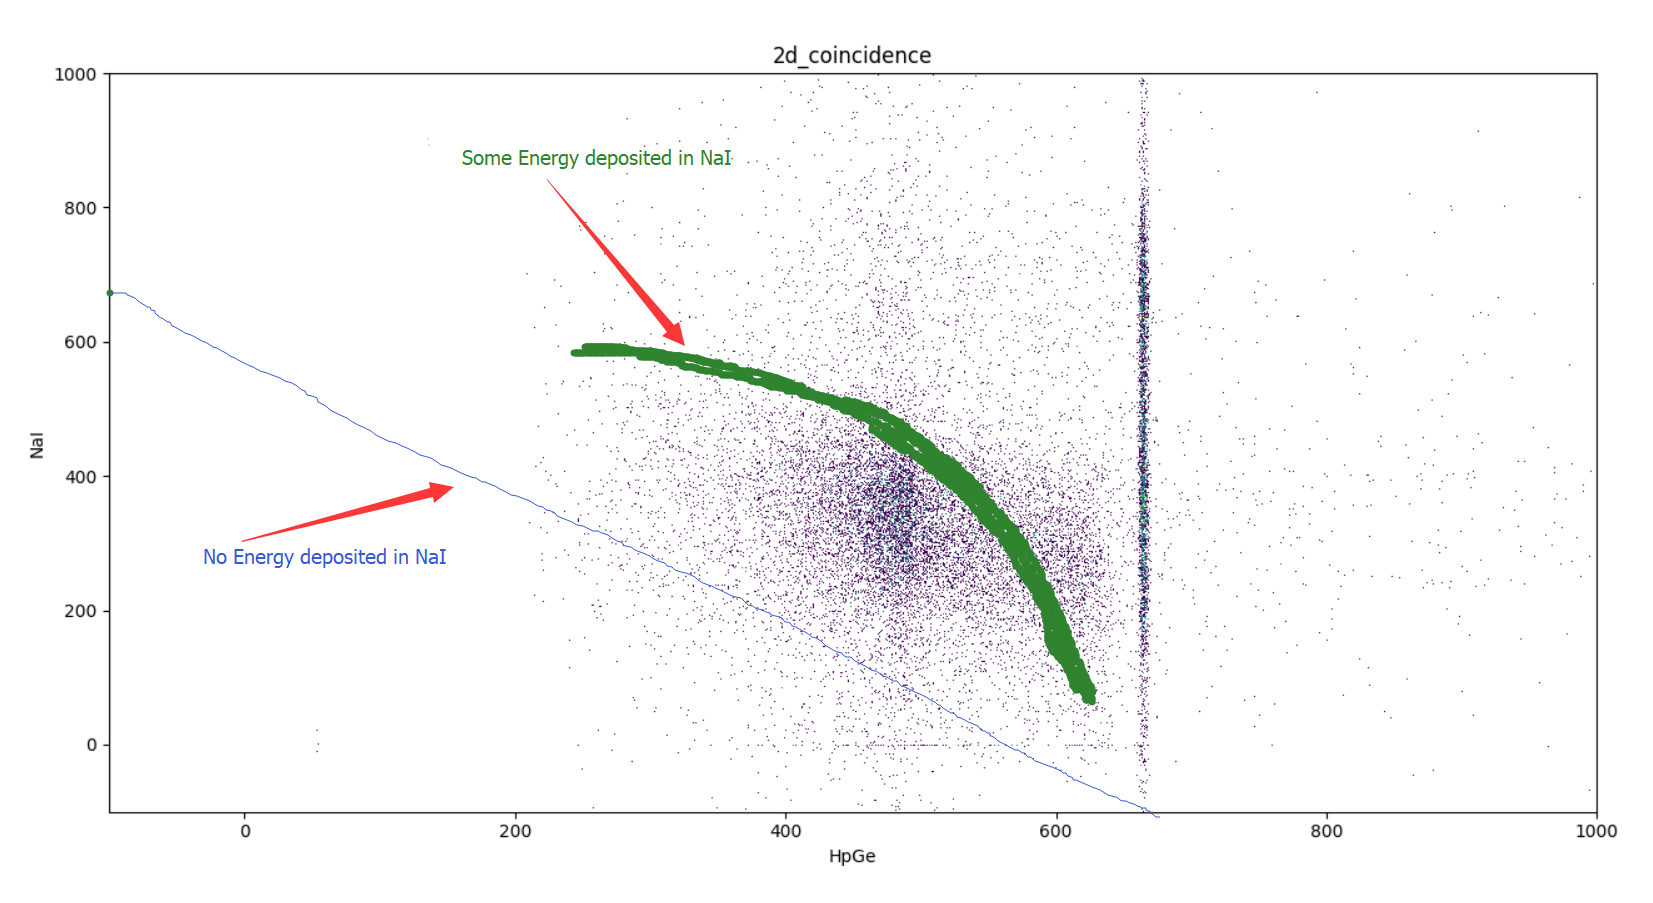
\includegraphics[width=0.7\linewidth, height=0.4\textheight]{pic/Coin_hist_2nd_Geo_expected_coin}
		\caption{The Expected Coincidence Data}
		\label{fig:coinhist2ndgeoexpectedcoin}
	\end{figure}\\
	The reason of curved line is that the energy capacity of NaI crystal at different energy level is not the same, which is a experimental result for crystals but not always true.	
	\section{Conclusion}
	\subsection{The Compton Scattering }
	The experiment for HpGe detector calibration and the Compton scattering is pretty successful, we get the expected energy distribution of Compton scattering. There are some waveform differences out of the the following reasons:\\
	1) There are some energy deposited in NaI(Tl) crystal;\\
	2) The simulation regard NaI crystal as a point and only consider first order approximation (i.e. Only scatter one time.);
	
	
	\section{Reference}
	\begin{thebibliography}{9}
		%\cite{Collar:2013gu}
		\bibitem{Collar:2013gu} 
		J.~I.~Collar,
		``Quenching and channeling of nuclear recoils in NaI(Tl): Implications for dark-matter searches,''
		Phys.\ Rev.\ C {\bf 88}, no. 3, 035806 (2013)
		doi:10.1103/PhysRevC.88.035806
		[arXiv:1302.0796 [physics.ins-det]].
		%%CITATION = doi:10.1103/PhysRevC.88.035806;%%
		%50 citations counted in INSPIRE as of 22 Oct 2017
		%\cite{Froborg:2016ova}
		
		\bibitem{Froborg:2016ova} 
		F.~Froborg [SABRE Collaboration],
		``SABRE: WIMP modulation detection in the northern and southern hemisphere,''
		J.\ Phys.\ Conf.\ Ser.\  {\bf 718}, no. 4, 042021 (2016)
		doi:10.1088/1742-6596/718/4/042021
		[arXiv:1601.05307 [physics.ins-det]].
		%%CITATION = doi:10.1088/1742-6596/718/4/042021;%%
		%8 citations counted in INSPIRE as of 22 Oct 2017
		
		%\cite{Peter:2012rz}
		\bibitem{Peter:2012rz} 
		A.~H.~G.~Peter,
		``Dark Matter: A Brief Review,''
		arXiv:1201.3942 [astro-ph.CO].
		%%CITATION = ARXIV:1201.3942;%%
		%30 citations counted in INSPIRE as of 22 Oct 2017
		
		\bibitem{website} 
		\texttt{https://physics.nist.gov}
		
		\bibitem{website}
		\texttt{http://www.spectrumtechniques.com}
		
	\end{thebibliography}
	
	
	\section{Appendix}
	\subsection{Simulation Code}
	The python 3 code for distribution simulation:
	\begin{lstlisting}
	#THE COMPTON COINCIDENCE SIMULATION PYTHON 3 CODE
	import numpy as np
	import matplotlib.pyplot as plt
				
	r_0=2.818*1e-15 #classcal electron radius
	#E_incidence=356 #the energy of the gamma ray indence
	E_incidence=662 #The incidence gamma ray energy(kev)
	width_detector=5 #the width of the detector(cm)
	depth_detector=5#the depth of the detector(cm)
	Theta_mean=80#the mean angle of the scattering(degree)
	N=1000#number of simulation sample  intervals
	R_outgoing=10#unit cm
			
	def de_to_ra(theta): 
	#transfer of angle units
		return theta*np.pi/180
	def ra_to_de(phi):
		return phi*180/np.pi
	
	def scattering_energy(E_in,theta_C): 
	#eneregy unit:keV,theta_C unit radian
		return E_in/(1+E_in/511*(1-np.cos(theta_C)))
	
	def inter_angle(a,b):# inter angel of two vector a,b
		co=a*b/(np.sum(a**2,1)*np.sum(b**2,1))
		return np.arccos(co)
	
	def diff_Klein_Nishina(theta,E_in):
	#differential crosssection as function of scattering angle(radian)
		alpha=E_in/511
		A=(1/(1+alpha*(1-np.cos(theta))))**2
		B=1+(np.cos(theta))**2
		C=1+(alpha**2*(1-np.cos(theta))**2)/(B*(1+alpha*(1-np.cos(theta))))
		diff_cros_sect=r_0**2*A*B/2*C
		E_out=scattering_energy(E_in,theta)
		return diff_cros_sect,E_out
	
	def coef_mu(E_gamma):
	'''The HpGe detecor efficiency coefficient '''
		a=5.28707
		b=-0.05223
		c=3.7691*1e-5
		mu=np.exp(a+b*E_gamma+c*E_gamma**2)
		return mu
	
	def angle_range(R_out,width):
	'''the angle range for a certain shape of HpGe detector'''
		return 2*np.arctan(width/(2*R_out))
	
	'''Consider the geometry of the cylinder detector, 
	I diveded the angles into different part to help me 
	to calculate the interatioc depth, by the formula of 
	piecewise function.	'''
	def depth_part1(theta,width,R,theta_tot):
		theta1=theta_tot/2-theta
		t=(width/2-R*np.tan(theta1))/np.sin(theta1)
		return t
	def depth_part2(theta,depth,theta_tot):
		theta2=theta_tot/2-theta
		t=depth/np.cos(theta2)
		return t
	def depth_part3(theta,width,R,theta_tot):
		theta3=theta-theta_tot/2
		t=(width/2-R*np.tan(theta3))/np.sin(theta3)
		return t
	def depth_t(R_out,depth,width,n): 
		'''here n is the number of discrete samples for simulation,
		This function input is the main angle, depth of detector,
		width of detector; 
		output is interaction depth of HpGe as function of theta'''
		t_depth=[]
		theta_tot=angle_range(R_out,width)
		t_cut=np.arctan(width/(2*(R_out+depth)))
		t_all=np.linspace(0,theta_tot,n)
		theta_1=t_all[t_all<(theta_tot/2-t_cut)]
		theta_2=t_all[t_all>(theta_tot/2-t_cut)]
		theta_2=theta_2[theta_2<(theta_tot/2+t_cut)]
		theta_3=t_all[t_all>(theta_tot/2+t_cut)]
		t_depth.extend(depth_part1(theta_1,width,R_out,theta_tot))
		t_depth.extend(depth_part2(theta_2,depth,theta_tot))
		t_depth.extend(depth_part3(theta_3,width,R_out,theta_tot))
		return t_depth
	
	def prob_inter(theta,width,depth,R_out):
	#the probability of gamma ray interaction with Ge detector.
		n=len(theta)
		E_out=scattering_energy(E_incidence,theta)
		mu=coef_mu(E_out)
		t=depth_t(R_out,depth,width,n)
		p=1-np.exp(-mu*t)
		return p
	
	def reative_diff_cs(theta,E_in):
	#calculate the relative cross section
		d=diff_Klein_Nishina(theta,E_in)
		d_max=max(d[0])
		return d[0]/d_max
	
	def det_E_distribution(theta_main,E_in,R_out,width,depth,n):
	'''Calculate the overall relative distribution and plot it'''
		delt_theta=angle_range(R_out,width)/2
		theta_LtoG=np.linspace(theta_main-delt_theta,theta_main+delt_theta,n)
		E_out=scattering_energy(E_in,theta_LtoG)
		p=prob_inter(theta_LtoG,width,depth,R_out)
		re_diff_cs=reative_diff_cs(theta_LtoG,E_in)
		dis=p*re_diff_cs
		dis=dis/max(dis)
		fig1 = plt.figure()
		ax = fig1.add_subplot(111)
		ax.plot(E_out,(dis)[::-1])
		ax.set_title('compton scaterring')
		ax.set_xlabel("Scatterred energy(keV)")
		ax.set_ylabel("probability distribution")
		plt.show(fig1)
	
	theta_main=de_to_ra(90)
	det_E_distribution(theta_main,E_incidence,R_outgoing,\
			\depth_detector,width_detector,N)
	
	'''This figure1 part is for calculating and plotting 
	Scattered energy in angle (0,180)deg.''' 		
	THETA=np.linspace(0,180,N)
	E_after_scatter=scattering_energy(E_incidence,de_to_ra(THETA))
	fig1 = plt.figure()
	ax = fig1.add_subplot(111)
	ax.plot(THETA, E_after_scatter)
	ax.set_title('compton scaterring Energy')
	ax.set_xlabel("Theta_C/deg")
	ax.set_ylabel("Scatterd Energy/Kev")
	plt.show(fig1)
	
	'''This figure2 part is for calculating the relative defferential 
	crossing section as function of theta.'''
	Theta_cross=np.linspace(0,180,N)
	prob,E_outgoing=diff_Klein_Nishina(de_to_ra(Theta_cross),E_incidence)
	fig2=plt.figure()
	ax1=fig2.add_subplot(111)
	ax1.plot(Theta_cross,prob/max(prob),'-r')
	ax1.set_title('compton scaterring diff cross section')
	ax1.set_xlabel("Theta_C/deg")
	ax1.set_ylabel("Relative Diff cross section")
	plt.show()
	
	'''This figure3 part for calculating the relative defferential 
	crossing section as function of scattered energy.'''
	fig3=plt.figure()
	ax2=fig3.add_subplot(111)
	ax2.plot(E_outgoing,prob/prob[-1],'-b')
	ax2.set_title('compton scaterring diff cross section')
	ax2.set_xlabel("Outgoing energy/keV")
	ax2.set_ylabel("Relative Diff cross section")
	#ax1.plot(Theta_cross,E_outgoing,'-b')
	plt.show(fig3)
	
	fig1.savefig('scattered_energy.png')
	fig2.savefig('theta_relative_diff_cross_section.png')
	fig3.savefig('energy_relative_diff_cross_section.png')
	\end{lstlisting}
	\subsection{The Data Analysis code}
	The python 3 code for data analysis:\\
	\textbf{Remark: Part of the binary file unpack code is from Jack Livingston (u5559529), who is also  ANU undergraduate and created the binary file unpack code last semester.}
	\begin{lstlisting}
	#DIGITIZER DATA EXTRACT AND ANALYSIS PYTHON 3 CODE		
	from struct import *
	from statistics import *
	from pylab import *
	import matplotlib.pyplot as plt
	from matplotlib.colors import LogNorm
	
	def header(x,num):
	'''Operation :
	Takes the headers out of a data set x, contains metadata
	Input:
	x=data set
	Output:
	set of headers for the data
	'''
		q = len(x)
		k = int(q / num)
		iterh = [0.0] * k
		C = [0.0] * k
		for i in range(k):
			iterh[i] = iter_unpack('l', x[0 + (i * num):20 \
				\+ (i * num)])
			C[i] = [inner for outer in iterh[i] for inner in outer]
		return C
	
	def wavedata(x,num,l=10):
	'''Operation:
	Takes the data out of a data set x
	Input:
	x=data set
	l: cosider that the memory of my laptop os not 
	enough for especially big size data file, I just 
	deal with 1/l of the data to get the characteristic.
	Output:
	list of  each waveform as list.
	'''
		q = len(x)
		k = int(q / (num*l))
		iterd = [0.0] * k
		C = [0.0] * k
		for j in range(k):
			iterd[j] = iter_unpack('h', x[24 + (j * num):num \
				\+ (j * num)])
			C[j] = [inner for outer in iterd[j] for inner in outer]
		return C
	def integ(H,K):
	'''Operation:
	Takes away background from an event's data, sums 
	the remaining data and then adds it to a new set
	Input:
	x=data set
	K: number of channels before the minof waveform,
	help to calculate the baseline average.
	Output:
	The integrated uncalibreted energy of each waveform
	as a list of lists.
	'''
		q=len(H)
		C=[0.0]*q
		D=[0.0]*q
		for i in range(q):
			avg=mean(H[i][0:argmin(H[i])-K])
			C[i]=H[i][argmin(H[i])-K:]-array(avg)
			D[i]=sum(C[i])
		return D
	
	def NaI(filename,cal_num):
	'''The operation function of NaI(Tl) detector data
	Input:
	filename:the filename of NaI data
	cal_number:the number of waveforms we actural calculate.
	Output:
		the integrated HpGe uncalibrated energy distribution
	'''
		file0=open(filename,'rb')
		X0=file0.read()
		file0.close()
		num_sam0=unpack('l',X0[0:4])[0]
		head0=header(X0,num_sam0)
		del head0
		wave0=wavedata(X0,num_sam0)
		del X0
		del num_sam0
		int_cal0=integ(wave0[0:cal_num],K=10)
		return int_cal0
	
	def HpGe(filename,cal_num):
	'''integration for NaI-mode HpGe data file
	Input:filename
	cal_num:actural calculating wavform number
	Output:
	the integrated HpGe uncalibrated energy distribution.
	'''
		file0=open(filename,'rb')
		X0=file0.read()
		file0.close()
		num_sam0=unpack('l',X0[0:4])[0]
		head0=header(X0,num_sam0)
		del head0
		wave0=wavedata(X0,num_sam0)
		del X0
		del num_sam0
		int_cal0=integ(wave0[0:cal_num],K=10)
		return int_cal0
		
	def HpGe_inted(filename,cal_num):
	'''caculation for hardware-intergrated HpGe data
	input:
	filename:
	filename of hardware-integrated HpGe data
	cal_num:
	actural calculating wavform number
	'''
		file1= open(filename, 'rb')
		X1 = file1.read()
		file1.close()
		num_sam1 = unpack('l', X1[0:4])[0]
		head1 = header(X1, num_sam1)
		del head1
		wave1 = wavedata(X1, num_sam1)
		del X1
		del num_sam1
		int_cal1 = np.max(wave1[0:cal_num], axis=1)
		#plot(wave1[0])
		#show()
		return int_cal1
		
	#calibration of HpGe data result
	re_HpGe=np.array(re_HpGe)*356.0/947
	#calibration of NaI data result
	re_NaI=np.array(re_NaI)*356.0/(-2750)
			
	#plot the histgram of NaI 
	figure()
	h0=hist(re_NaI,bins=1100,range=(-20000,70000))
	xlabel('energy')
	ylabel('account')
	title('NaI')
	#histgram for HpGe
	figure()
	h1=hist(re_HpGe,bins=2000,range=(0,1000))
	title('HpGe')
	xlabel('HpGe_energy')
	ylabel('counts')
	
	#plot the data from both detector together
	figure()
	plt.hist2d(re_HpGe,re_NaI,bins=(1200,1200),\
		\range=((-100,1000),(-100,1000)),norm=LogNorm())
	plt.title('2d_coincidence')
	
	show()
	
	
	\end{lstlisting}

\end{document}
